%%%%%%%%%%%%%%%%%%%%%%%%%%%%%%%%%%%%%%%%%%%%%%%%%%%%%%%%%%%%%%%%%%%%%%%%%
% Deep Reinforcement Learning for EV Routing Optimization
% Professional Beamer Presentation
% Authors: Salem Fradi & Dhia Elhak Ezzeddini
% Supervisor: Dr. Ferdaoues Chaabane
% Academic Year: 2025-2026
%%%%%%%%%%%%%%%%%%%%%%%%%%%%%%%%%%%%%%%%%%%%%%%%%%%%%%%%%%%%%%%%%%%%%%%%%

\documentclass[aspectratio=169,11pt]{beamer}

%-------------------------------------------------------------------------
% THEME AND COLORS
%-------------------------------------------------------------------------
\usetheme{Madrid}
\usecolortheme{whale}

% Custom colors
\definecolor{primaryblue}{RGB}{0,84,147}
\definecolor{secondaryblue}{RGB}{0,119,182}
\definecolor{accentgreen}{RGB}{0,150,136}
\definecolor{lightgray}{RGB}{245,245,245}
\definecolor{darkgray}{RGB}{60,60,60}

\setbeamercolor{palette primary}{bg=primaryblue,fg=white}
\setbeamercolor{palette secondary}{bg=secondaryblue,fg=white}
\setbeamercolor{palette tertiary}{bg=primaryblue,fg=white}
\setbeamercolor{structure}{fg=primaryblue}
\setbeamercolor{title}{fg=white,bg=primaryblue}
\setbeamercolor{frametitle}{fg=white,bg=primaryblue}
\setbeamercolor{block title}{bg=primaryblue,fg=white}
\setbeamercolor{block body}{bg=lightgray,fg=darkgray}
\setbeamercolor{block title alerted}{bg=red!70!black,fg=white}
\setbeamercolor{block title example}{bg=accentgreen,fg=white}

%-------------------------------------------------------------------------
% PACKAGES
%-------------------------------------------------------------------------
\usepackage[utf8]{inputenc}
\usepackage[T1]{fontenc}
\usepackage{amsmath,amsfonts,amssymb}
\usepackage{graphicx}
\usepackage{booktabs}
\usepackage{tikz}
\usepackage{pgfplots}
\usepackage{xcolor}
\usepackage{hyperref}
\usepackage{caption}
\usepackage{subcaption}
\usepackage{array}
\usepackage{multirow}
\usepackage{fontawesome5}
\usepackage{pifont}

\usetikzlibrary{shapes,arrows,positioning,calc,decorations.pathreplacing,fit,backgrounds}
\pgfplotsset{compat=1.17}

%-------------------------------------------------------------------------
% CUSTOM COMMANDS
%-------------------------------------------------------------------------
\newcommand{\cmark}{\ding{51}}
\newcommand{\xmark}{\ding{55}}
\newcommand{\highlight}[1]{\textcolor{accentgreen}{\textbf{#1}}}
\newcommand{\emphbox}[1]{\colorbox{lightgray}{\textbf{#1}}}

%-------------------------------------------------------------------------
% FOOTER AND NAVIGATION
%-------------------------------------------------------------------------
\setbeamertemplate{navigation symbols}{}
\setbeamertemplate{footline}{
    \leavevmode%
    \hbox{%
        \begin{beamercolorbox}[wd=.333333\paperwidth,ht=2.25ex,dp=1ex,center]{author in head/foot}%
            \usebeamerfont{author in head/foot}\insertshortauthor
        \end{beamercolorbox}%
        \begin{beamercolorbox}[wd=.333333\paperwidth,ht=2.25ex,dp=1ex,center]{title in head/foot}%
            \usebeamerfont{title in head/foot}\insertshorttitle
        \end{beamercolorbox}%
        \begin{beamercolorbox}[wd=.333333\paperwidth,ht=2.25ex,dp=1ex,right]{date in head/foot}%
            \usebeamerfont{date in head/foot}\insertshortdate{}\hspace*{2em}
            \insertframenumber{} / \inserttotalframenumber\hspace*{2ex}
        \end{beamercolorbox}}%
    \vskip0pt%
}

%-------------------------------------------------------------------------
% TITLE INFORMATION
%-------------------------------------------------------------------------
\title[DRL for EV Routing]{Deep Reinforcement Learning for\\Electric Vehicle Routing Optimization}
\subtitle{Energy-Minimizing Electric Vehicle Routing Problem (EM-EVRP)}
\author[D. Ezzeddini \& S. Fradi]{Dhia Elhak Ezzeddini \and Salem Fradi}
\institute[Sup'Com]{
    Higher School of Communication of Tunis\\
    Carthage University\\[0.3cm]
    \textbf{Supervisor:} Dr. Ferdaoues Chaabane\\
    \textbf{Host Company:} Sagemcom
}
\date{Academic Year 2025--2026}

%-------------------------------------------------------------------------
% GRAPHICS PATH
%-------------------------------------------------------------------------
\graphicspath{{../docs/figures/}{../images/}}

%=========================================================================
% DOCUMENT BEGINS
%=========================================================================
\begin{document}

%-------------------------------------------------------------------------
% TITLE SLIDE
%-------------------------------------------------------------------------
\begin{frame}[plain]
    \titlepage
\end{frame}

%-------------------------------------------------------------------------
% OUTLINE
%-------------------------------------------------------------------------
\begin{frame}{Outline}
    \tableofcontents[hideallsubsections]
\end{frame}

%=========================================================================
\section{Introduction}
%=========================================================================

%-------------------------------------------------------------------------
\begin{frame}{Context: The Rise of Electric Vehicles}
    \begin{columns}[T]
        \begin{column}{0.55\textwidth}
            \textbf{Global EV Adoption Trends:}
            \begin{itemize}
                \item Global EV sales exceeded \textbf{14 million} in 2023
                \item Expected to reach \textbf{40+ million} by 2030
                \item Major push from governments and corporations
            \end{itemize}
            
            \vspace{0.5cm}
            \textbf{Key Drivers:}
            \begin{itemize}
                \item \highlight{Climate change} mitigation goals
                \item Stricter \highlight{emission regulations}
                \item Decreasing \highlight{battery costs}
                \item Government \highlight{incentives} and subsidies
            \end{itemize}
        \end{column}
        \begin{column}{0.42\textwidth}
            \begin{block}{Why EVs for Logistics?}
                \begin{itemize}
                    \item Lower operating costs
                    \item Zero tailpipe emissions
                    \item Urban delivery restrictions
                    \item Corporate sustainability
                \end{itemize}
            \end{block}
            
            \vspace{0.3cm}
            \begin{alertblock}{Challenge}
                Limited range \& charging infrastructure require \textbf{smart routing}
            \end{alertblock}
        \end{column}
    \end{columns}
\end{frame}

%-------------------------------------------------------------------------
\begin{frame}{Challenges in EV Logistics}
    \begin{center}
        \begin{tikzpicture}[
            challenge/.style={rectangle, rounded corners, draw=primaryblue, fill=lightgray, 
                             text width=3.5cm, minimum height=1.5cm, align=center, font=\small},
            arrow/.style={->, thick, primaryblue}
        ]
            % Central node
            \node[ellipse, draw=primaryblue, fill=primaryblue!20, text width=2.5cm, 
                  align=center, font=\bfseries] (center) {EV Logistics\\Challenges};
            
            % Challenge nodes
            \node[challenge] (range) at (-5,2) {\faIcon{battery-half}\\Limited\\Driving Range};
            \node[challenge] (charge) at (-5,-2) {\faIcon{charging-station}\\Sparse Charging\\Infrastructure};
            \node[challenge] (time) at (0,3) {\faIcon{clock}\\Long Charging\\Duration};
            \node[challenge] (energy) at (5,2) {\faIcon{bolt}\\Variable Energy\\Consumption};
            \node[challenge] (plan) at (5,-2) {\faIcon{route}\\Complex Route\\Planning};
            \node[challenge] (cost) at (0,-3) {\faIcon{dollar-sign}\\Operational\\Cost Optimization};
            
            % Arrows
            \draw[arrow] (center) -- (range);
            \draw[arrow] (center) -- (charge);
            \draw[arrow] (center) -- (time);
            \draw[arrow] (center) -- (energy);
            \draw[arrow] (center) -- (plan);
            \draw[arrow] (center) -- (cost);
        \end{tikzpicture}
    \end{center}
\end{frame}

%-------------------------------------------------------------------------
\begin{frame}{Motivation: Why This Project?}
    \begin{columns}[T]
        \begin{column}{0.48\textwidth}
            \begin{block}{Industry Needs}
                \begin{itemize}
                    \item Growing demand for \textbf{sustainable logistics}
                    \item Need for \textbf{real-time} routing decisions
                    \item Integration with \textbf{smart city} infrastructure
                    \item \textbf{Cost reduction} through energy optimization
                \end{itemize}
            \end{block}
        \end{column}
        \begin{column}{0.48\textwidth}
            \begin{block}{Technical Gaps}
                \begin{itemize}
                    \item Traditional VRP methods \textbf{don't scale}
                    \item Energy models often \textbf{oversimplified}
                    \item Limited \textbf{real-world} deployment tools
                    \item Need for \textbf{learning-based} approaches
                \end{itemize}
            \end{block}
        \end{column}
    \end{columns}
    
    \vspace{0.5cm}
    \begin{exampleblock}{Our Contribution}
        \centering
        An \textbf{end-to-end solution} combining Deep Reinforcement Learning with\\
        physics-based energy modeling and real-world deployment infrastructure
    \end{exampleblock}
\end{frame}

%=========================================================================
\section{Problem Statement}
%=========================================================================

%-------------------------------------------------------------------------
\begin{frame}{Electric Vehicle Routing Problem (EVRP)}
    \begin{columns}[T]
        \begin{column}{0.55\textwidth}
            \textbf{Classical VRP:}
            \begin{itemize}
                \item Serve all customers from depot
                \item Minimize total travel distance/cost
                \item Respect vehicle capacity
            \end{itemize}
            
            \vspace{0.3cm}
            \textbf{EVRP Extension:}
            \begin{itemize}
                \item \highlight{Battery capacity} constraints
                \item \highlight{Charging station} visits allowed
                \item \highlight{Energy consumption} varies with load
                \item \highlight{Recharging time} impacts schedule
            \end{itemize}
        \end{column}
        \begin{column}{0.42\textwidth}
            \begin{center}
                \begin{tikzpicture}[scale=0.7, every node/.style={scale=0.7}]
                    % Depot
                    \node[rectangle, draw=red, fill=red!30, minimum size=0.6cm] (depot) at (0,0) {\faIcon{warehouse}};
                    \node[below=0.1cm of depot, font=\tiny] {Depot};
                    
                    % Charging stations
                    \node[circle, draw=accentgreen, fill=accentgreen!30, minimum size=0.5cm] (cs1) at (-2,2) {\faIcon{plug}};
                    \node[circle, draw=accentgreen, fill=accentgreen!30, minimum size=0.5cm] (cs2) at (2,-1.5) {\faIcon{plug}};
                    
                    % Customers
                    \node[circle, draw=primaryblue, fill=primaryblue!30, minimum size=0.4cm] (c1) at (-1.5,-1) {};
                    \node[circle, draw=primaryblue, fill=primaryblue!30, minimum size=0.4cm] (c2) at (1,2) {};
                    \node[circle, draw=primaryblue, fill=primaryblue!30, minimum size=0.4cm] (c3) at (2.5,1) {};
                    \node[circle, draw=primaryblue, fill=primaryblue!30, minimum size=0.4cm] (c4) at (-2,-2) {};
                    \node[circle, draw=primaryblue, fill=primaryblue!30, minimum size=0.4cm] (c5) at (0.5,-2.5) {};
                    
                    % Routes
                    \draw[->, thick, red!70] (depot) -- (c1);
                    \draw[->, thick, red!70] (c1) -- (c4);
                    \draw[->, thick, red!70] (c4) -- (cs1);
                    \draw[->, thick, red!70] (cs1) -- (c2);
                    \draw[->, thick, red!70] (c2) -- (depot);
                    
                    \draw[->, thick, blue!70, dashed] (depot) -- (c3);
                    \draw[->, thick, blue!70, dashed] (c3) -- (c5);
                    \draw[->, thick, blue!70, dashed] (c5) -- (cs2);
                    \draw[->, thick, blue!70, dashed] (cs2) -- (depot);
                    
                    % Legend
                    \node[font=\tiny] at (0, -3.5) {Multiple routes with charging stops};
                \end{tikzpicture}
            \end{center}
        \end{column}
    \end{columns}
\end{frame}

%-------------------------------------------------------------------------
\begin{frame}{Energy-Minimizing EVRP (EM-EVRP)}
    \begin{block}{Problem Definition}
        \textbf{Objective:} Minimize \textbf{total energy consumption} while serving all customers
    \end{block}
    
    \vspace{0.3cm}
    \textbf{Subject to Constraints:}
    
    \begin{columns}[T]
        \begin{column}{0.48\textwidth}
            \begin{enumerate}
                \item \textbf{Customer Service}
                \begin{itemize}
                    \item Each customer visited exactly once
                    \item Full demand satisfaction
                \end{itemize}
                
                \item \textbf{Vehicle Capacity}
                \begin{itemize}
                    \item Total load $\leq$ max capacity
                    \item Partial deliveries possible
                \end{itemize}
                
                \item \textbf{Battery SOC}
                \begin{itemize}
                    \item SOC $\geq 0$ at all times
                    \item Recharge at stations
                \end{itemize}
            \end{enumerate}
        \end{column}
        \begin{column}{0.48\textwidth}
            \begin{enumerate}
                \setcounter{enumi}{3}
                \item \textbf{Time Windows}
                \begin{itemize}
                    \item Service within $[a_i, b_i]$
                    \item Route time budget
                \end{itemize}
                
                \item \textbf{Route Feasibility}
                \begin{itemize}
                    \item Start and end at depot
                    \item Valid path existence
                \end{itemize}
                
                \item \textbf{Charging Logic}
                \begin{itemize}
                    \item Optional station visits
                    \item Charging time cost
                \end{itemize}
            \end{enumerate}
        \end{column}
    \end{columns}
\end{frame}

%-------------------------------------------------------------------------
\begin{frame}{Why Minimize Energy Instead of Distance?}
    \begin{columns}[T]
        \begin{column}{0.48\textwidth}
            \begin{alertblock}{Distance $\neq$ Energy}
                Shortest path may not be most energy-efficient!
            \end{alertblock}
            
            \vspace{0.3cm}
            \textbf{Energy depends on:}
            \begin{itemize}
                \item \highlight{Vehicle load} (heavier = more energy)
                \item \highlight{Road gradient} (uphill = more energy)
                \item \highlight{Speed profile} (higher speed = more drag)
                \item \highlight{Regenerative braking} (downhill = energy recovery)
            \end{itemize}
        \end{column}
        \begin{column}{0.48\textwidth}
            \begin{exampleblock}{Energy Optimization Benefits}
                \begin{itemize}
                    \item \textbf{Extended range} per charge
                    \item \textbf{Fewer charging} stops needed
                    \item \textbf{Lower operational} costs
                    \item \textbf{Reduced battery} degradation
                    \item More \textbf{sustainable} operations
                \end{itemize}
            \end{exampleblock}
        \end{column}
    \end{columns}
    
    \vspace{0.5cm}
    \begin{center}
        \fbox{\parbox{0.8\textwidth}{\centering
            \textbf{Key Insight:} A longer route going downhill may consume\\
            less energy than a shorter uphill route!
        }}
    \end{center}
\end{frame}

%=========================================================================
\section{Mathematical Formulation}
%=========================================================================

%-------------------------------------------------------------------------
\begin{frame}{MILP Formulation: Sets and Parameters}
    \begin{columns}[T]
        \begin{column}{0.48\textwidth}
            \begin{block}{Sets}
                \begin{tabular}{cl}
                    $N$ & All nodes (depot + customers) \\
                    $C$ & Customers $C = N \setminus \{0\}$ \\
                    $S$ & Charging stations \\
                    $K$ & Fleet of vehicles \\
                    $R$ & Trip indices
                \end{tabular}
            \end{block}
            
            \vspace{0.3cm}
            \begin{block}{Network Parameters}
                \begin{tabular}{cl}
                    $d_i$ & Demand at customer $i$ \\
                    $Q_k$ & Capacity of vehicle $k$ \\
                    $t_{ij}$ & Travel time on arc $(i,j)$ \\
                    $[a_i, b_i]$ & Time window at node $i$
                \end{tabular}
            \end{block}
        \end{column}
        \begin{column}{0.48\textwidth}
            \begin{block}{EV Energy Parameters}
                \begin{tabular}{cl}
                    $m_c$ & Vehicle curb mass \\
                    $C_d$ & Aerodynamic drag coeff. \\
                    $C_r$ & Rolling resistance coeff. \\
                    $\rho$ & Air density \\
                    $A$ & Frontal area \\
                    $\alpha_{ij}$ & Slope angle on arc \\
                    $\varphi_{d/r}$ & Motor efficiency \\
                    $\phi_{d/r}$ & Battery efficiency
                \end{tabular}
            \end{block}
        \end{column}
    \end{columns}
\end{frame}

%-------------------------------------------------------------------------
\begin{frame}{Physics-Based Energy Consumption Model}
    \begin{block}{Total Vehicle Mass on Arc $(i,j)$}
        \[
        m_{ij} = m_c + u_{ij}
        \]
        where $u_{ij}$ is the current cargo load
    \end{block}
    
    \begin{block}{Mechanical Power Required}
        \[
        P_{ij} = \underbrace{\frac{1}{2} C_d \rho A v_{ij}^2}_{\text{Aerodynamic drag}} + 
                 \underbrace{m_{ij} g \sin\alpha_{ij}}_{\text{Gravitational}} + 
                 \underbrace{m_{ij} g C_r \cos\alpha_{ij}}_{\text{Rolling resistance}}
        \]
    \end{block}
    
    \begin{block}{Energy Consumption with Efficiency}
        \[
        E_{ij} = \begin{cases}
            \phi_d \cdot \varphi_d \cdot P_{ij} \cdot t_{ij} & \text{if } P_{ij} \geq 0 \text{ (propulsion)} \\[0.2cm]
            \phi_r \cdot \varphi_r \cdot P_{ij} \cdot t_{ij} & \text{if } P_{ij} < 0 \text{ (regeneration)}
        \end{cases}
        \]
    \end{block}
\end{frame}

%-------------------------------------------------------------------------
\begin{frame}{MILP Formulation: Objective and Constraints}
    \begin{block}{Objective Function}
        \[
        \min \sum_{k \in K} \sum_{r \in R} \sum_{(i,j) \in A} E_{ij} \cdot x_{ijk}^r
        \]
        Minimize total energy consumption across all routes
    \end{block}
    
    \vspace{0.3cm}
    \begin{columns}[T]
        \begin{column}{0.48\textwidth}
            \textbf{Customer Service:}
            \[
            \sum_{k \in K} \sum_{r \in R} y_{ik}^r = 1, \quad \forall i \in C
            \]
            
            \textbf{Capacity:}
            \[
            \sum_{i \in C} d_i \cdot y_{ik}^r \leq Q_k, \quad \forall k, r
            \]
        \end{column}
        \begin{column}{0.48\textwidth}
            \textbf{Flow Conservation:}
            \[
            \sum_j x_{ijk}^r = y_{ik}^r = \sum_j x_{jik}^r
            \]
            
            \textbf{Subtour Elimination (MTZ):}
            \[
            w_{ik}^r - w_{jk}^r + |C| x_{ijk}^r \leq |C| - 1
            \]
        \end{column}
    \end{columns}
    
    \vspace{0.3cm}
    \begin{center}
        \textcolor{red}{\textbf{NP-Hard Problem}} $\Rightarrow$ Exact methods don't scale to large instances
    \end{center}
\end{frame}

%=========================================================================
\section{Baseline Optimization Methods}
%=========================================================================

%-------------------------------------------------------------------------
\begin{frame}{Classical Optimization Approaches}
    We implemented \textbf{four baseline methods} for comparison:
    
    \vspace{0.5cm}
    \begin{columns}[T]
        \begin{column}{0.48\textwidth}
            \begin{block}{1. Google OR-Tools}
                \begin{itemize}
                    \item Industry-standard solver
                    \item Constraint programming
                    \item Arc cost callbacks for energy
                    \item Local search improvements
                \end{itemize}
            \end{block}
            
            \begin{block}{2. Hill Climbing}
                \begin{itemize}
                    \item Simple local search
                    \item 2-opt, Or-opt, Exchange
                    \item Fast but local optima
                \end{itemize}
            \end{block}
        \end{column}
        \begin{column}{0.48\textwidth}
            \begin{block}{3. Simulated Annealing}
                \begin{itemize}
                    \item Probabilistic acceptance
                    \item Escapes local optima
                    \item Temperature-based control
                    \item $P(\text{accept}) = e^{-\Delta E/T}$
                \end{itemize}
            \end{block}
            
            \begin{block}{4. Ant Colony Optimization}
                \begin{itemize}
                    \item Nature-inspired
                    \item Pheromone trails
                    \item Collective intelligence
                    \item Good for combinatorial
                \end{itemize}
            \end{block}
        \end{column}
    \end{columns}
\end{frame}

%-------------------------------------------------------------------------
\begin{frame}{Metaheuristics: Local Search Operators}
    \begin{center}
        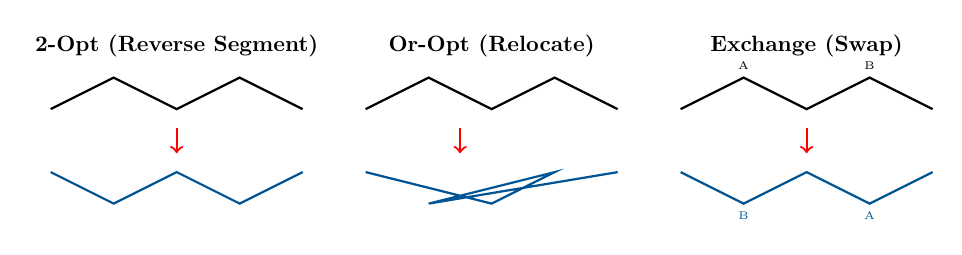
\begin{tikzpicture}[scale=0.8, every node/.style={scale=0.8}]
            % 2-opt
            \node[font=\bfseries] at (-5, 2.5) {2-Opt (Reverse Segment)};
            \draw[thick] (-7,1.5) -- (-6,2) -- (-5,1.5) -- (-4,2) -- (-3,1.5);
            \draw[thick, primaryblue] (-7,0.5) -- (-6,0) -- (-5,0.5) -- (-4,0) -- (-3,0.5);
            \draw[->, thick, red] (-5, 1.2) -- (-5, 0.8);
            
            % Or-opt
            \node[font=\bfseries] at (0, 2.5) {Or-Opt (Relocate)};
            \draw[thick] (-2,1.5) -- (-1,2) -- (0,1.5) -- (1,2) -- (2,1.5);
            \draw[thick, primaryblue] (-2,0.5) -- (0,0) -- (1,0.5) -- (-1,0) -- (2,0.5);
            \draw[->, thick, red] (-0.5, 1.2) -- (-0.5, 0.8);
            
            % Exchange
            \node[font=\bfseries] at (5, 2.5) {Exchange (Swap)};
            \draw[thick] (3,1.5) -- (4,2) node[above, font=\tiny] {A} -- (5,1.5) -- (6,2) node[above, font=\tiny] {B} -- (7,1.5);
            \draw[thick, primaryblue] (3,0.5) -- (4,0) node[below, font=\tiny] {B} -- (5,0.5) -- (6,0) node[below, font=\tiny] {A} -- (7,0.5);
            \draw[->, thick, red] (5, 1.2) -- (5, 0.8);
        \end{tikzpicture}
    \end{center}
    
    \vspace{0.5cm}
    \begin{block}{Simulated Annealing Acceptance Rule}
        \[
        P(\text{accept worse solution}) = \exp\left(-\frac{\Delta E}{T}\right)
        \]
        \begin{itemize}
            \item High temperature $\Rightarrow$ explore (accept worse solutions)
            \item Low temperature $\Rightarrow$ exploit (only accept improvements)
            \item Cooling schedule: $T_{k+1} = \alpha \cdot T_k$ where $\alpha \in [0.9, 0.99]$
        \end{itemize}
    \end{block}
\end{frame}

%-------------------------------------------------------------------------
\begin{frame}{Ant Colony Optimization}
    \begin{columns}[T]
        \begin{column}{0.55\textwidth}
            \textbf{Probabilistic Transition Rule:}
            \[
            p_{ij}^a = \frac{[\tau_{ij}]^\alpha \cdot [\eta_{ij}]^\beta}{\sum_{l \in \mathcal{N}_i} [\tau_{il}]^\alpha \cdot [\eta_{il}]^\beta}
            \]
            
            where:
            \begin{itemize}
                \item $\tau_{ij}$ = pheromone level on arc $(i,j)$
                \item $\eta_{ij} = 1/c_{ij}$ = heuristic information
                \item $\alpha, \beta$ = importance parameters
            \end{itemize}
            
            \vspace{0.3cm}
            \textbf{Pheromone Update:}
            \[
            \tau_{ij} \leftarrow (1-\rho)\tau_{ij} + \sum_a \Delta\tau_{ij}^a
            \]
            
            Better solutions deposit more pheromone
        \end{column}
        \begin{column}{0.42\textwidth}
            \begin{center}
                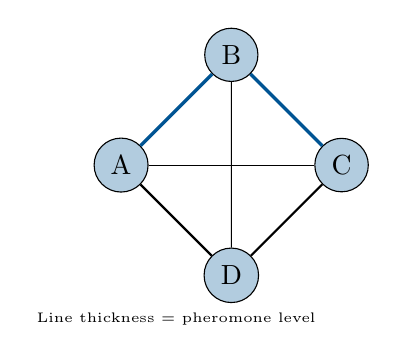
\begin{tikzpicture}[scale=0.7]
                    \node[circle, draw, fill=primaryblue!30] (A) at (0,0) {A};
                    \node[circle, draw, fill=primaryblue!30] (B) at (2,2) {B};
                    \node[circle, draw, fill=primaryblue!30] (C) at (4,0) {C};
                    \node[circle, draw, fill=primaryblue!30] (D) at (2,-2) {D};
                    
                    \draw[very thick, primaryblue] (A) -- (B);
                    \draw[thick] (A) -- (D);
                    \draw[very thick, primaryblue] (B) -- (C);
                    \draw[thin] (A) -- (C);
                    \draw[thin] (B) -- (D);
                    \draw[thick] (C) -- (D);
                    
                    \node[font=\tiny] at (1, -2.8) {Line thickness = pheromone level};
                \end{tikzpicture}
            \end{center}
            
            \begin{block}{Key Properties}
                \begin{itemize}
                    \item Positive feedback
                    \item Parallel exploration
                    \item Emergent optimization
                \end{itemize}
            \end{block}
        \end{column}
    \end{columns}
\end{frame}

%=========================================================================
\section{Deep Reinforcement Learning Approach}
%=========================================================================

%-------------------------------------------------------------------------
\begin{frame}{Why Deep Reinforcement Learning?}
    \begin{columns}[T]
        \begin{column}{0.48\textwidth}
            \begin{alertblock}{Traditional Methods Limitations}
                \begin{itemize}
                    \item Exact methods: exponential time
                    \item Heuristics: problem-specific design
                    \item No generalization to new instances
                    \item Slow for real-time applications
                \end{itemize}
            \end{alertblock}
        \end{column}
        \begin{column}{0.48\textwidth}
            \begin{exampleblock}{DRL Advantages}
                \begin{itemize}
                    \item \textbf{Learn} to solve, not program
                    \item \textbf{Generalize} to new instances
                    \item \textbf{Fast inference} (milliseconds)
                    \item \textbf{End-to-end} optimization
                \end{itemize}
            \end{exampleblock}
        \end{column}
    \end{columns}
    
    \vspace{0.5cm}
    \begin{block}{Key Insight}
        \centering
        Train a neural network to \textbf{construct} solutions step-by-step,\\
        learning from experience which decisions lead to lower energy consumption
    \end{block}
    
    \vspace{0.3cm}
    \begin{center}
        \textbf{Inspired by:} Kool et al., ``Attention, Learn to Solve Routing Problems!'' (ICLR 2019)
    \end{center}
\end{frame}

%-------------------------------------------------------------------------
\begin{frame}{MDP Formulation for EVRP}
    \begin{block}{Markov Decision Process Components}
        \begin{description}
            \item[State $s_t$:] Current partial solution + vehicle status
                \begin{itemize}
                    \item Visited nodes, current position
                    \item Remaining capacity, SOC, time budget
                \end{itemize}
            \item[Action $a_t$:] Select next node to visit
                \begin{itemize}
                    \item Customer, charging station, or depot
                \end{itemize}
            \item[Reward $r_t$:] Negative energy for traversed arc
                \begin{itemize}
                    \item Minimize cumulative energy consumption
                \end{itemize}
            \item[Policy $\pi_\theta$:] Neural network with parameters $\theta$
                \begin{itemize}
                    \item Maps states to action probabilities
                \end{itemize}
        \end{description}
    \end{block}
    
    \vspace{0.3cm}
    \begin{center}
        \textbf{Objective:} $\max_\theta \mathbb{E}_{\pi_\theta}\left[\sum_t r_t\right] = \max_\theta \mathbb{E}_{\pi_\theta}\left[-\sum_t E_t\right]$
    \end{center}
\end{frame}

%-------------------------------------------------------------------------
\begin{frame}{Attention-Based Architecture: Overview}
    \begin{center}
        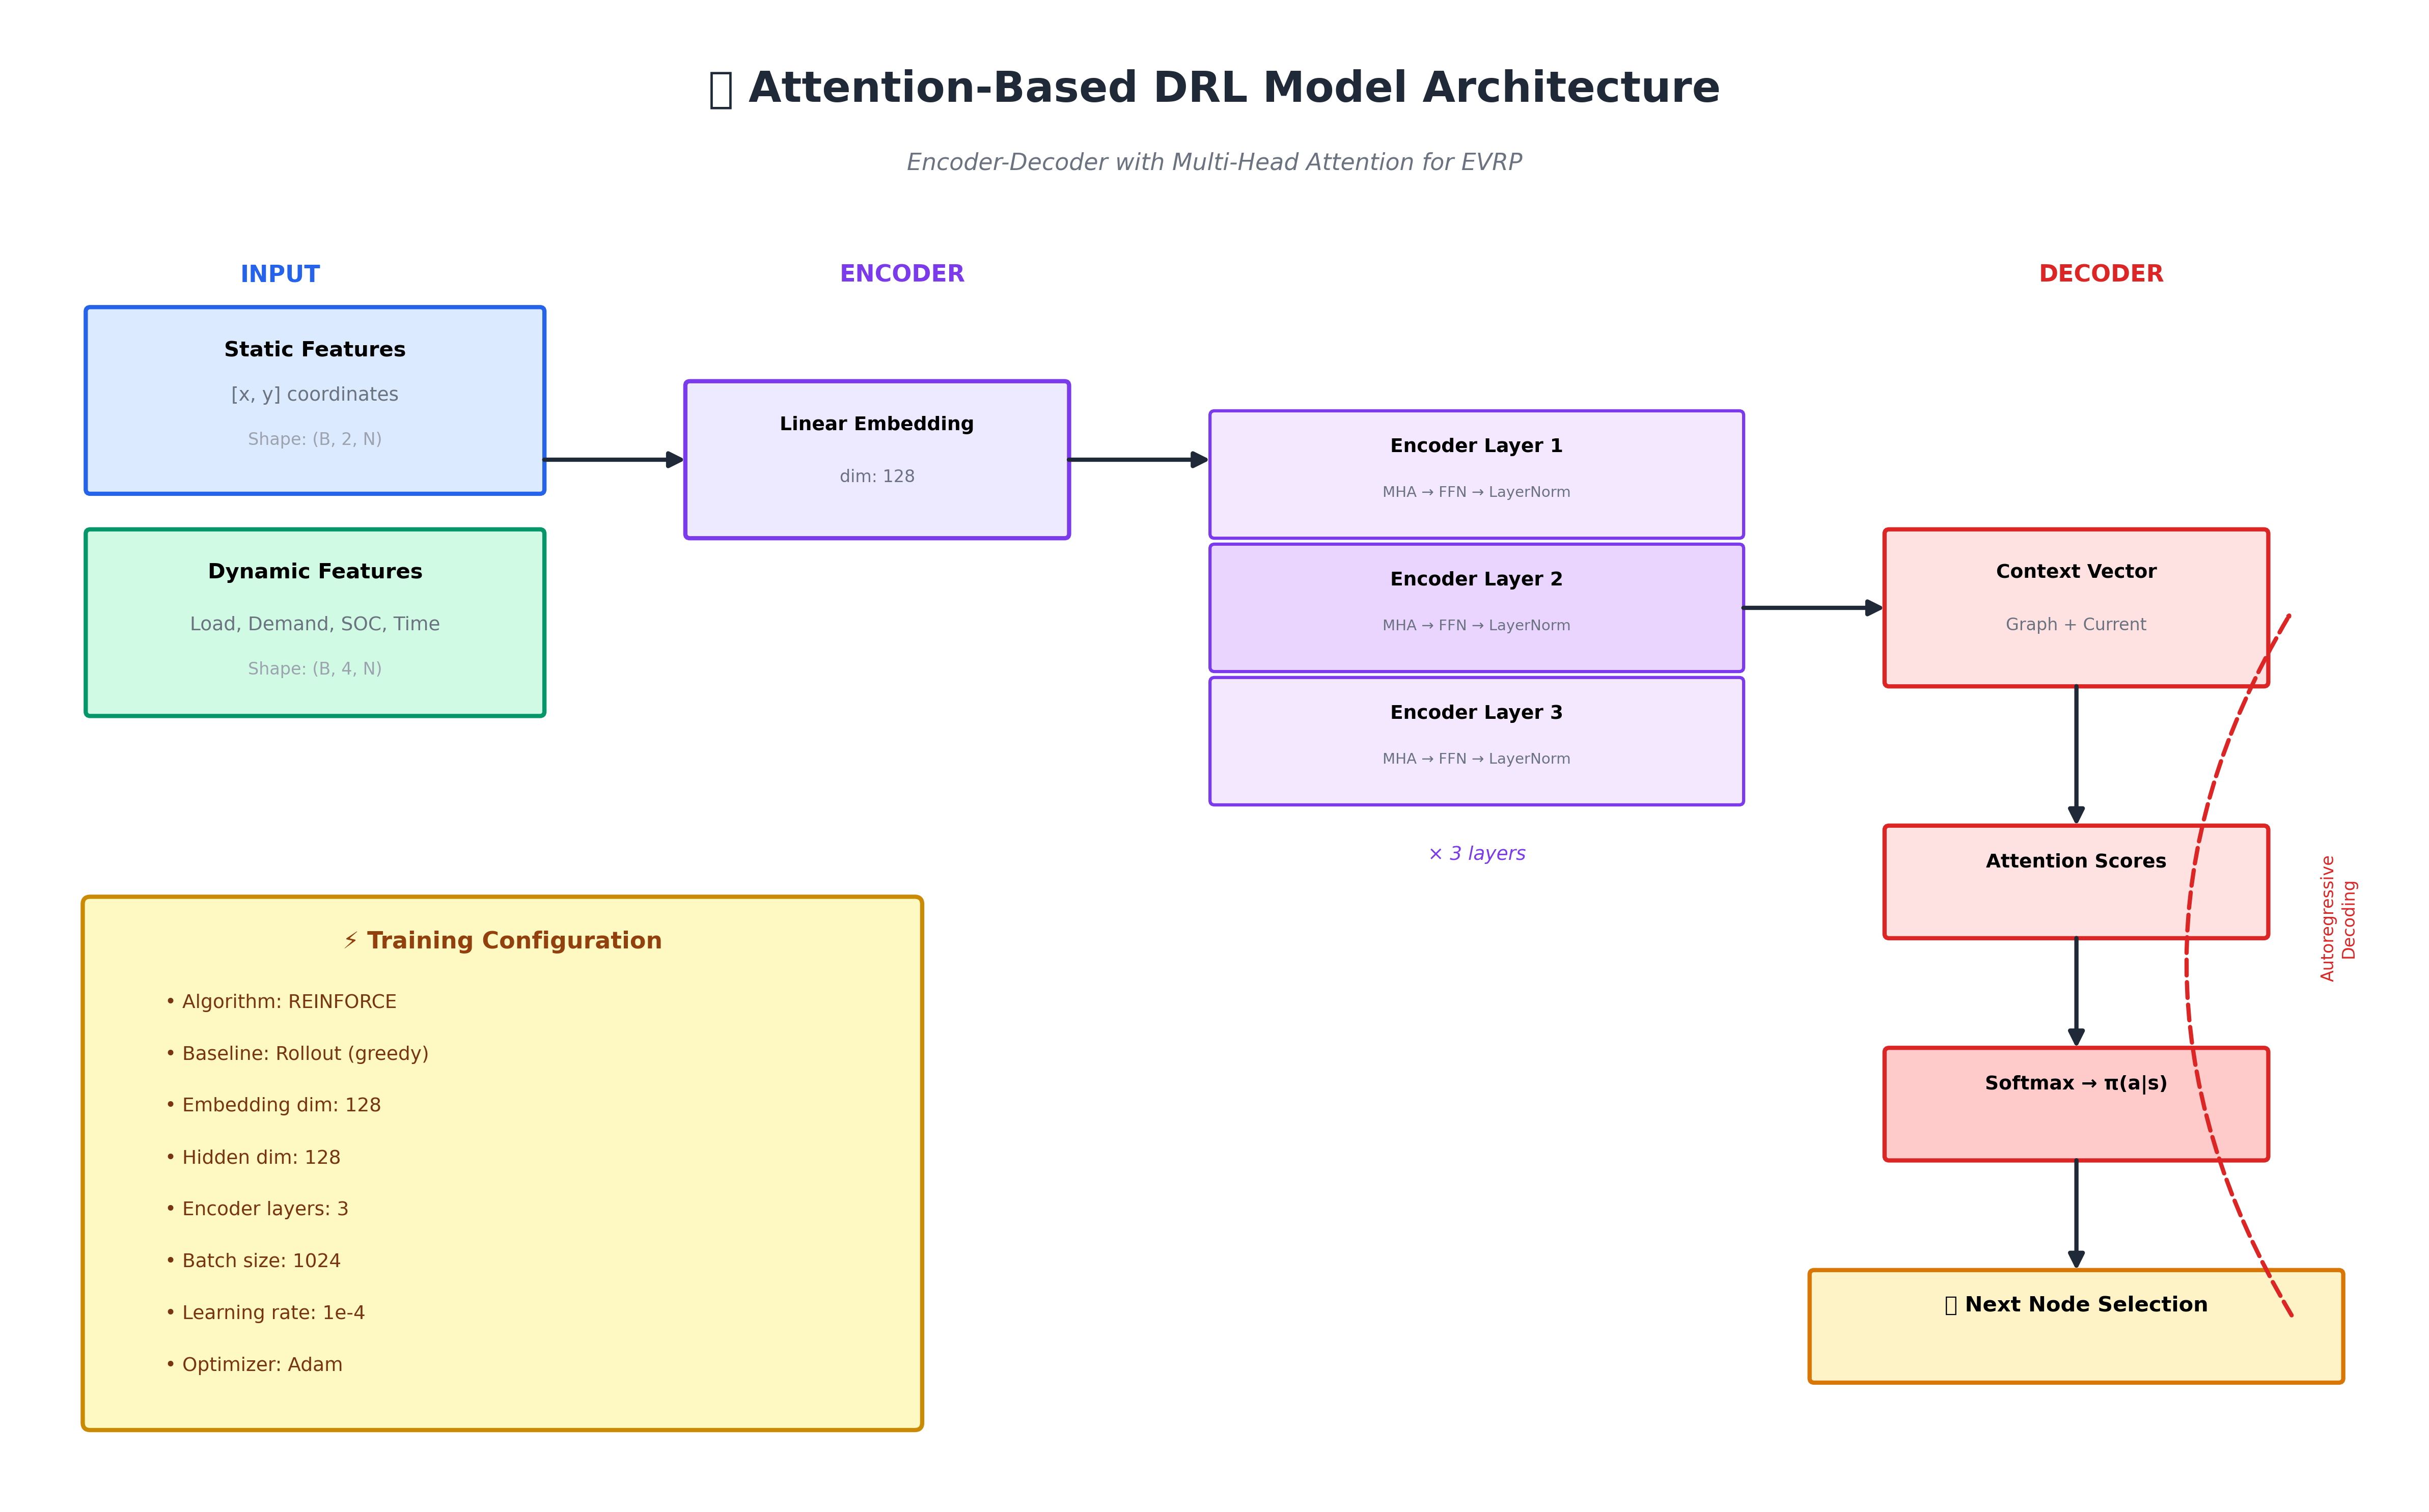
\includegraphics[width=0.70\textwidth]{drl_model_architecture.png}
    \end{center}
    
    \vspace{0.3cm}
    \begin{columns}[T]
        \begin{column}{0.48\textwidth}
            \begin{block}{Encoder}
                \begin{itemize}
                    \item Multi-head self-attention
                    \item Captures node relationships
                    \item Produces node embeddings
                \end{itemize}
            \end{block}
        \end{column}
        \begin{column}{0.48\textwidth}
            \begin{block}{Decoder}
                \begin{itemize}
                    \item Autoregressive generation
                    \item Context-aware selection
                    \item Masked attention for feasibility
                \end{itemize}
            \end{block}
        \end{column}
    \end{columns}
\end{frame}

%-------------------------------------------------------------------------
\begin{frame}{Graph Attention Encoder}
    \begin{block}{Multi-Head Self-Attention Layer}
        \[
        h_i^{(l)} = \text{BN}\left(h_i^{(l-1)} + \text{MHA}\left(h_i^{(l-1)}, H^{(l-1)}\right)\right)
        \]
    \end{block}
    
    \begin{columns}[T]
        \begin{column}{0.55\textwidth}
            \textbf{Attention Mechanism:}
            \[
            \text{Attention}(Q, K, V) = \text{softmax}\left(\frac{QK^T}{\sqrt{d_k}}\right)V
            \]
            
            \vspace{0.3cm}
            \textbf{Graph Embedding:}
            \[
            \bar{h} = \frac{1}{n}\sum_{i=1}^{n} h_i
            \]
            
            Mean aggregation of all node embeddings
        \end{column}
        \begin{column}{0.42\textwidth}
            \begin{block}{Architecture Details}
                \begin{tabular}{ll}
                    Embedding dim & 128 \\
                    Attention heads & 8 \\
                    Encoder layers & 3 \\
                    FF hidden & 512 \\
                    Normalization & Batch
                \end{tabular}
            \end{block}
        \end{column}
    \end{columns}
\end{frame}

%-------------------------------------------------------------------------
\begin{frame}{Context-Aware Decoder}
    \begin{block}{Context Embedding}
        \[
        c_t = W_c \left[\bar{h}; h_{\pi_{t-1}}; \text{load}_t; \text{SOC}_t; \text{time}_t\right]
        \]
        
        Combines: graph embedding + previous node + vehicle state
    \end{block}
    
    \begin{block}{Attention-Based Selection}
        \[
        u_{tj} = \begin{cases}
            C \cdot \tanh\left(\frac{q_t \cdot k_j}{\sqrt{d_k}}\right) & \text{if } j \in \mathcal{A}_t \\
            -\infty & \text{otherwise}
        \end{cases}
        \]
        \[
        p_\theta(a_t = j | s_t) = \text{softmax}(u_t)_j
        \]
    \end{block}
    
    \begin{exampleblock}{Feasibility Masking}
        $\mathcal{A}_t$ = nodes that satisfy: demand $\leq$ capacity AND energy needed $\leq$ SOC
    \end{exampleblock}
\end{frame}

%-------------------------------------------------------------------------
\begin{frame}{REINFORCE Training Algorithm}
    \begin{block}{Policy Gradient Objective}
        \[
        J(\theta) = \mathbb{E}_{\pi_\theta}\left[L(\pi)\right]
        \]
        where $L(\pi)$ is the total route energy consumption
    \end{block}
    
    \begin{block}{Gradient Estimation with Baseline}
        \[
        \nabla_\theta J \approx \frac{1}{B}\sum_{i=1}^{B} \left(L(\pi_i) - b(s_i)\right) \nabla_\theta \log p_\theta(\pi_i | s_i)
        \]
        
        \begin{itemize}
            \item $b(s)$ = baseline value (reduces variance)
            \item We use \textbf{rollout baseline}: greedy policy copy
        \end{itemize}
    \end{block}
    
    \begin{exampleblock}{Baseline Update Rule}
        Update baseline when current policy shows statistically significant improvement\\
        (paired t-test with $p < 0.05$ on validation instances)
    \end{exampleblock}
\end{frame}

%-------------------------------------------------------------------------
\begin{frame}{EV-Specific Model Features}
    \begin{columns}[T]
        \begin{column}{0.48\textwidth}
            \begin{block}{State of Charge Tracking}
                \[
                \text{SOC}_{t+1} = \text{SOC}_t - \frac{E_{ij}}{E_{\text{battery}}}
                \]
                
                \begin{itemize}
                    \item Continuous SOC monitoring
                    \item Reset at charging stations
                    \item Negative consumption = regeneration
                \end{itemize}
            \end{block}
            
            \begin{block}{Load Dynamics}
                \[
                \text{load}_{t+1} = \text{load}_t - d_{\text{served}}
                \]
                
                Cargo decreases after each delivery
            \end{block}
        \end{column}
        \begin{column}{0.48\textwidth}
            \begin{block}{Dynamic Masking Rules}
                \begin{enumerate}
                    \item Sufficient SOC for arc?
                    \item Can reach depot from there?
                    \item Enough capacity for demand?
                    \item Time budget remaining?
                    \item Station detour feasible?
                \end{enumerate}
            \end{block}
            
            \begin{alertblock}{Learning Charging Decisions}
                Model learns \textbf{when} to visit charging stations through experience
            \end{alertblock}
        \end{column}
    \end{columns}
\end{frame}

%=========================================================================
\section{System Architecture}
%=========================================================================

%-------------------------------------------------------------------------
\begin{frame}{End-to-End System Pipeline}
    \begin{center}
        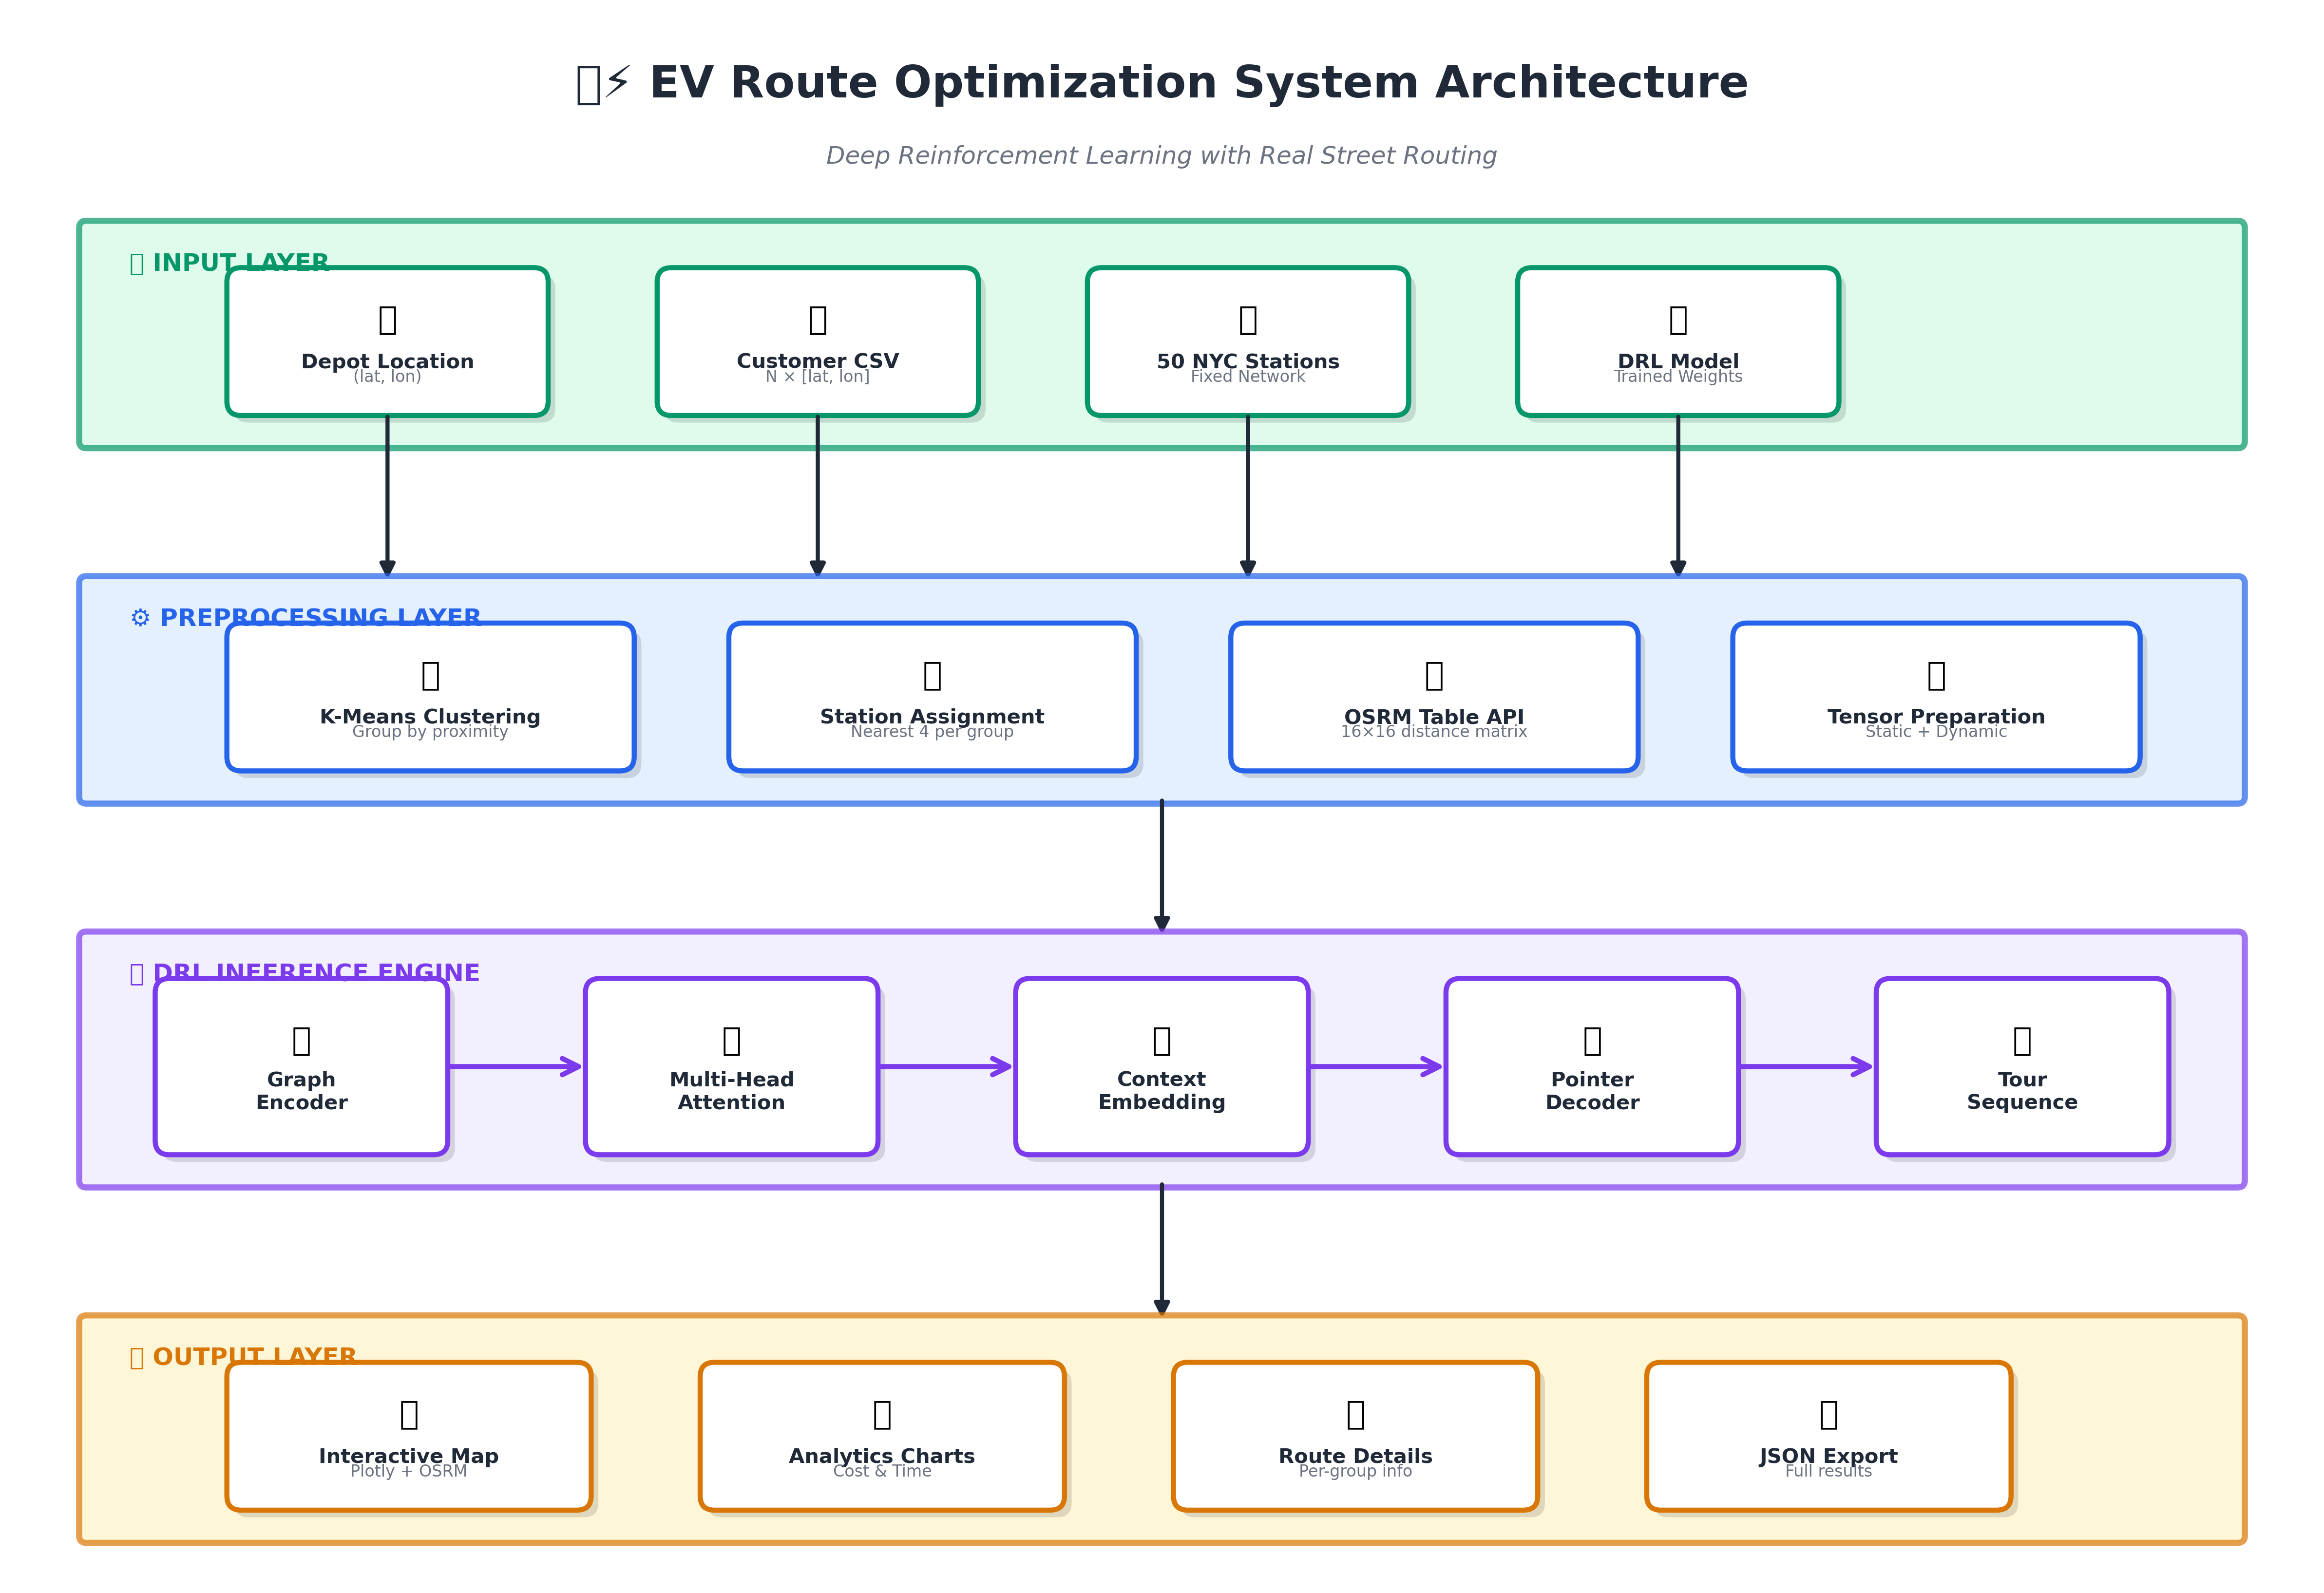
\includegraphics[width=0.75\textwidth]{system_architecture.png}
    \end{center}
\end{frame}

%-------------------------------------------------------------------------
\begin{frame}{Data Generation Pipeline}
    \begin{columns}[T]
        \begin{column}{0.55\textwidth}
            \textbf{Training Data Generation:}
            \begin{enumerate}
                \item \textbf{Random coordinates} for nodes
                    \begin{itemize}
                        \item Depot: [25,75] $\times$ [25,75]
                        \item Customers: [0,101] $\times$ [0,101]
                        \item Stations: quadrant-based placement
                    \end{itemize}
                \item \textbf{Random elevations} [0,101]
                    \begin{itemize}
                        \item Normalized for slope calculation
                    \end{itemize}
                \item \textbf{Random demands} [1, max\_demand]
                \item \textbf{Pairwise distances} and slopes
            \end{enumerate}
        \end{column}
        \begin{column}{0.42\textwidth}
            \begin{center}
                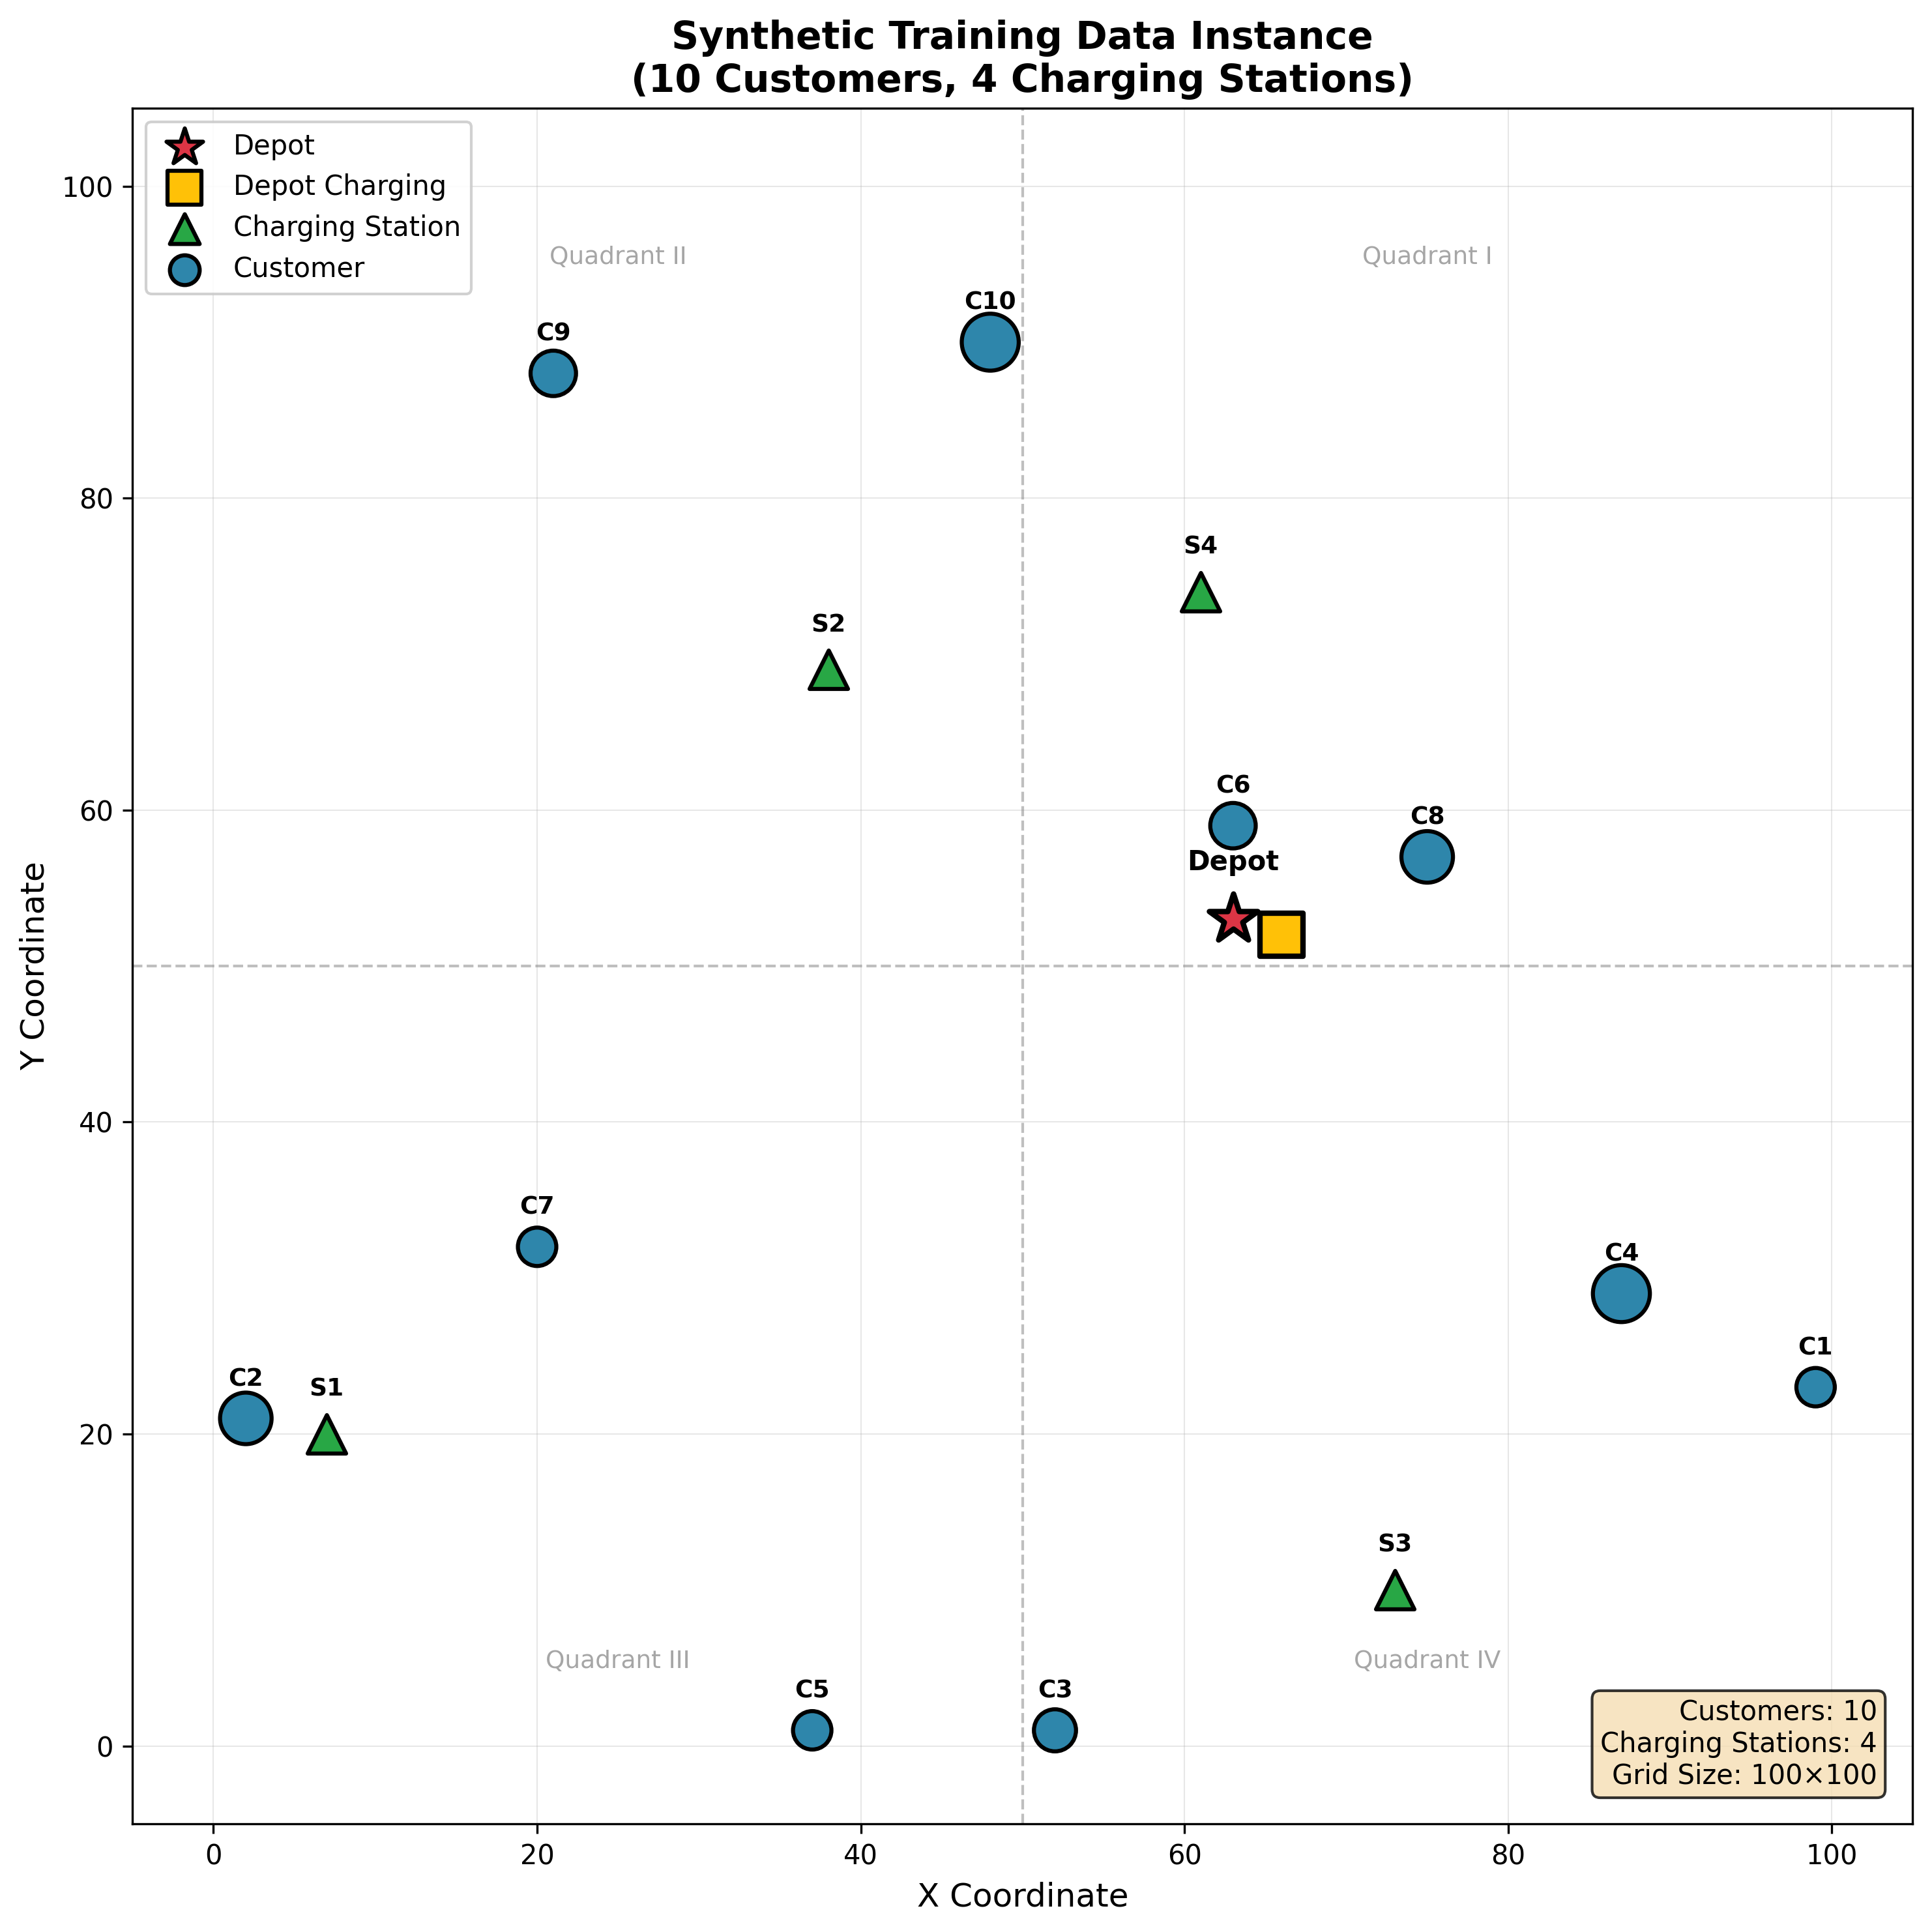
\includegraphics[width=\textwidth]{synthetic_training_data.png}
            \end{center}
            
            \begin{block}{Dataset Size}
                \begin{tabular}{ll}
                    Training & 1,280,000 \\
                    Validation & 10,000 \\
                    Batch size & 1,024
                \end{tabular}
            \end{block}
        \end{column}
    \end{columns}
\end{frame}

%-------------------------------------------------------------------------
\begin{frame}{Real-World Deployment: OSRM Integration}
    \begin{columns}[T]
        \begin{column}{0.55\textwidth}
            \textbf{Open Source Routing Machine (OSRM):}
            \begin{itemize}
                \item Production-grade routing engine
                \item Real street-level distances
                \item Fast table API for distance matrices
                \item OpenStreetMap data
            \end{itemize}
            
            \vspace{0.3cm}
            \textbf{Integration Pipeline:}
            \begin{enumerate}
                \item Upload customer GPS coordinates
                \item Query OSRM for distance matrix
                \item Run DRL model inference
                \item Reconstruct routes on map
                \item Calculate real energy consumption
            \end{enumerate}
        \end{column}
        \begin{column}{0.42\textwidth}
            \begin{block}{Scalability Strategy}
                \textbf{K-means Clustering:}
                \begin{itemize}
                    \item Group customers into batches
                    \item 10 customers per group
                    \item Run DRL on each group
                    \item Combine results
                \end{itemize}
            \end{block}
            
            \begin{exampleblock}{NYC Configuration}
                50 pre-configured charging stations across New York City
            \end{exampleblock}
        \end{column}
    \end{columns}
\end{frame}

%-------------------------------------------------------------------------
\begin{frame}{Interactive Dashboard: Main Interface}
    \begin{center}
        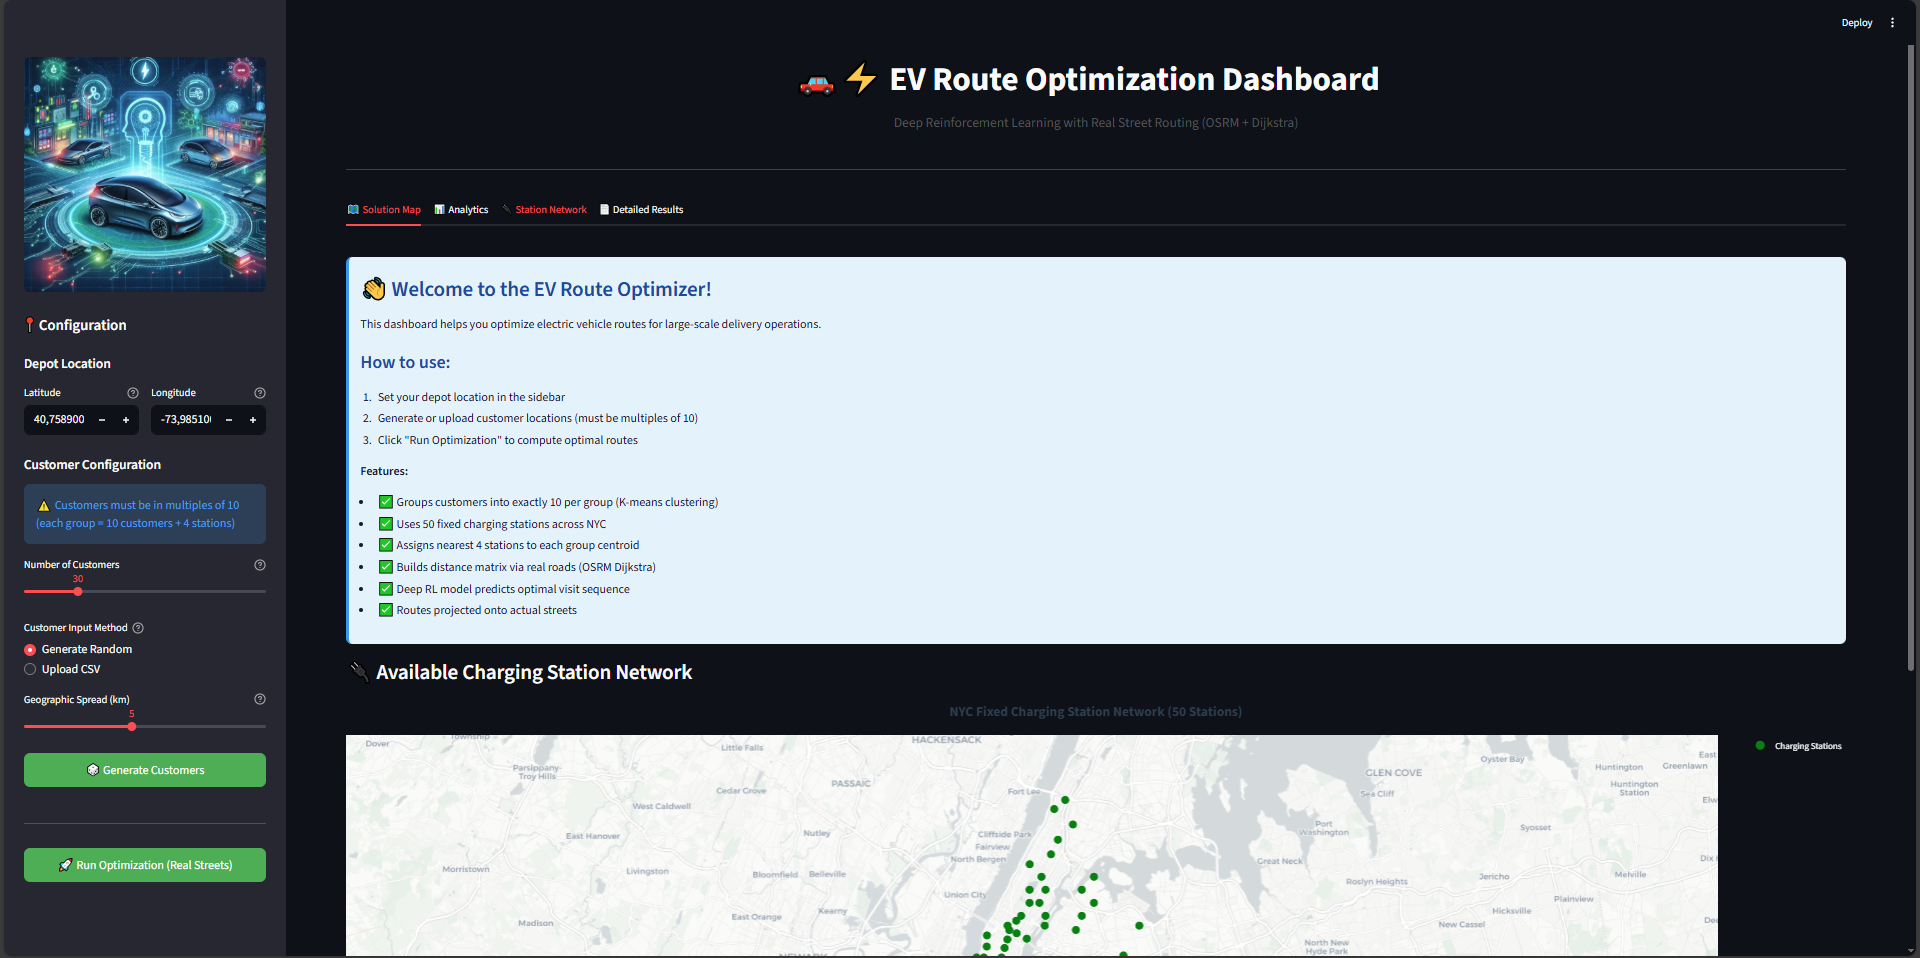
\includegraphics[width=0.85\textwidth]{main_page.PNG}
    \end{center}
    
    \begin{block}{Features}
        Upload customers $\bullet$ Configure EV parameters $\bullet$ Select charging stations $\bullet$ Real-time optimization
    \end{block}
\end{frame}

%-------------------------------------------------------------------------
\begin{frame}{Interactive Dashboard: Route Optimization}
    \begin{columns}
        \begin{column}{0.48\textwidth}
            \begin{center}
                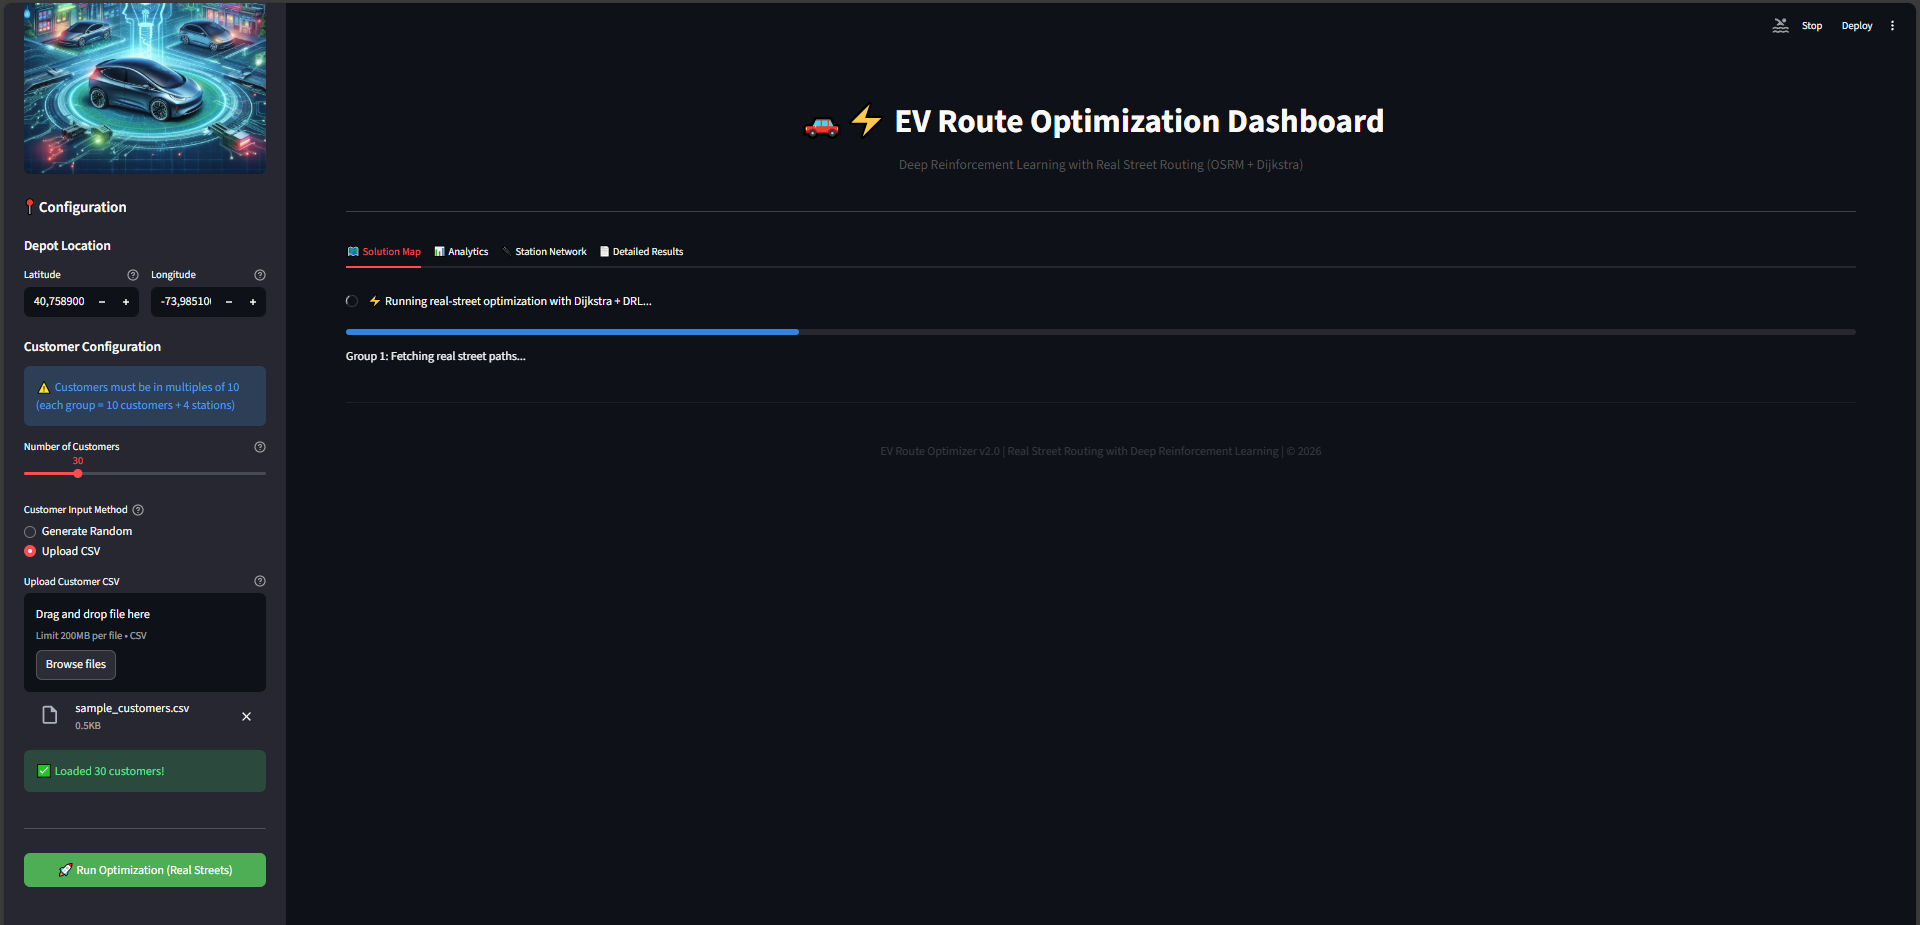
\includegraphics[width=\textwidth]{inference.PNG}
            \end{center}
            \begin{center}
                \small\textbf{Inference Process}
            \end{center}
        \end{column}
        \begin{column}{0.48\textwidth}
            \begin{center}
                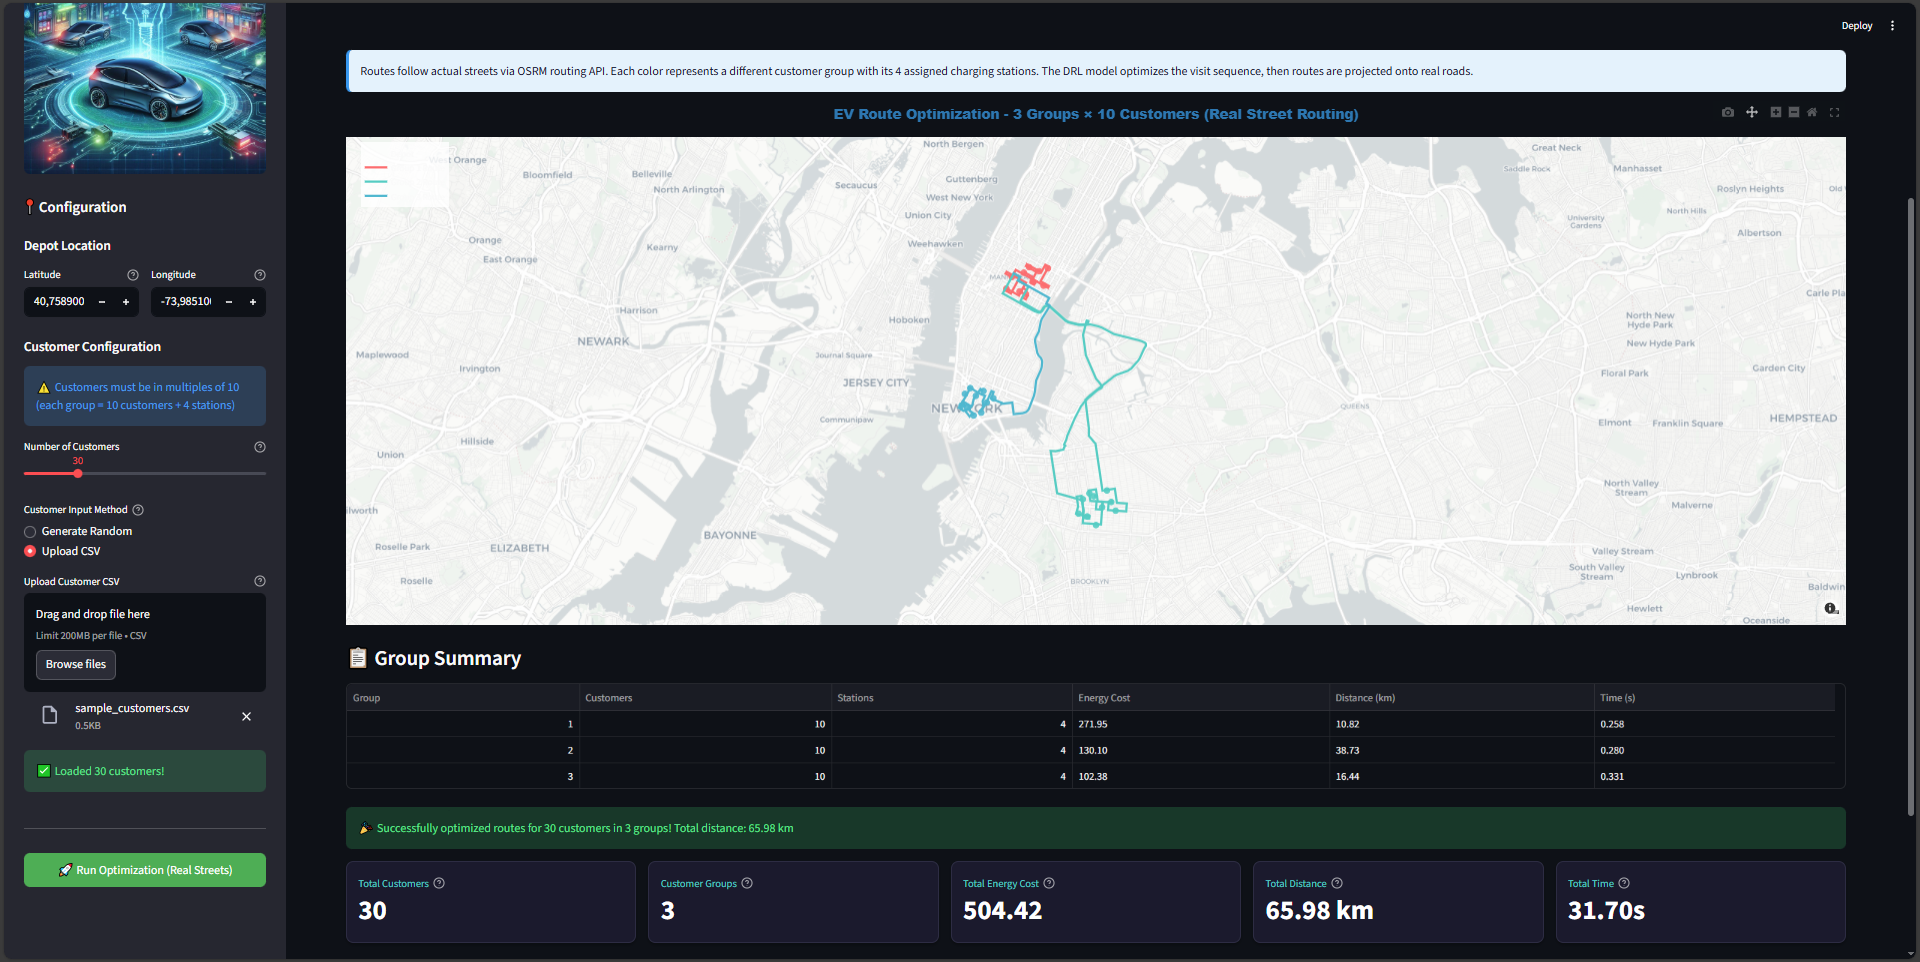
\includegraphics[width=\textwidth]{result.PNG}
            \end{center}
            \begin{center}
                \small\textbf{Optimized Routes}
            \end{center}
        \end{column}
    \end{columns}
    
    \vspace{0.3cm}
    \begin{itemize}
        \item Interactive map with customer locations and charging stations
        \item Real-time route visualization with street-level paths
        \item Color-coded routes for multiple vehicles
    \end{itemize}
\end{frame}

%-------------------------------------------------------------------------
\begin{frame}{Interactive Dashboard: Analytics}
    \begin{columns}
        \begin{column}{0.48\textwidth}
            \begin{center}
                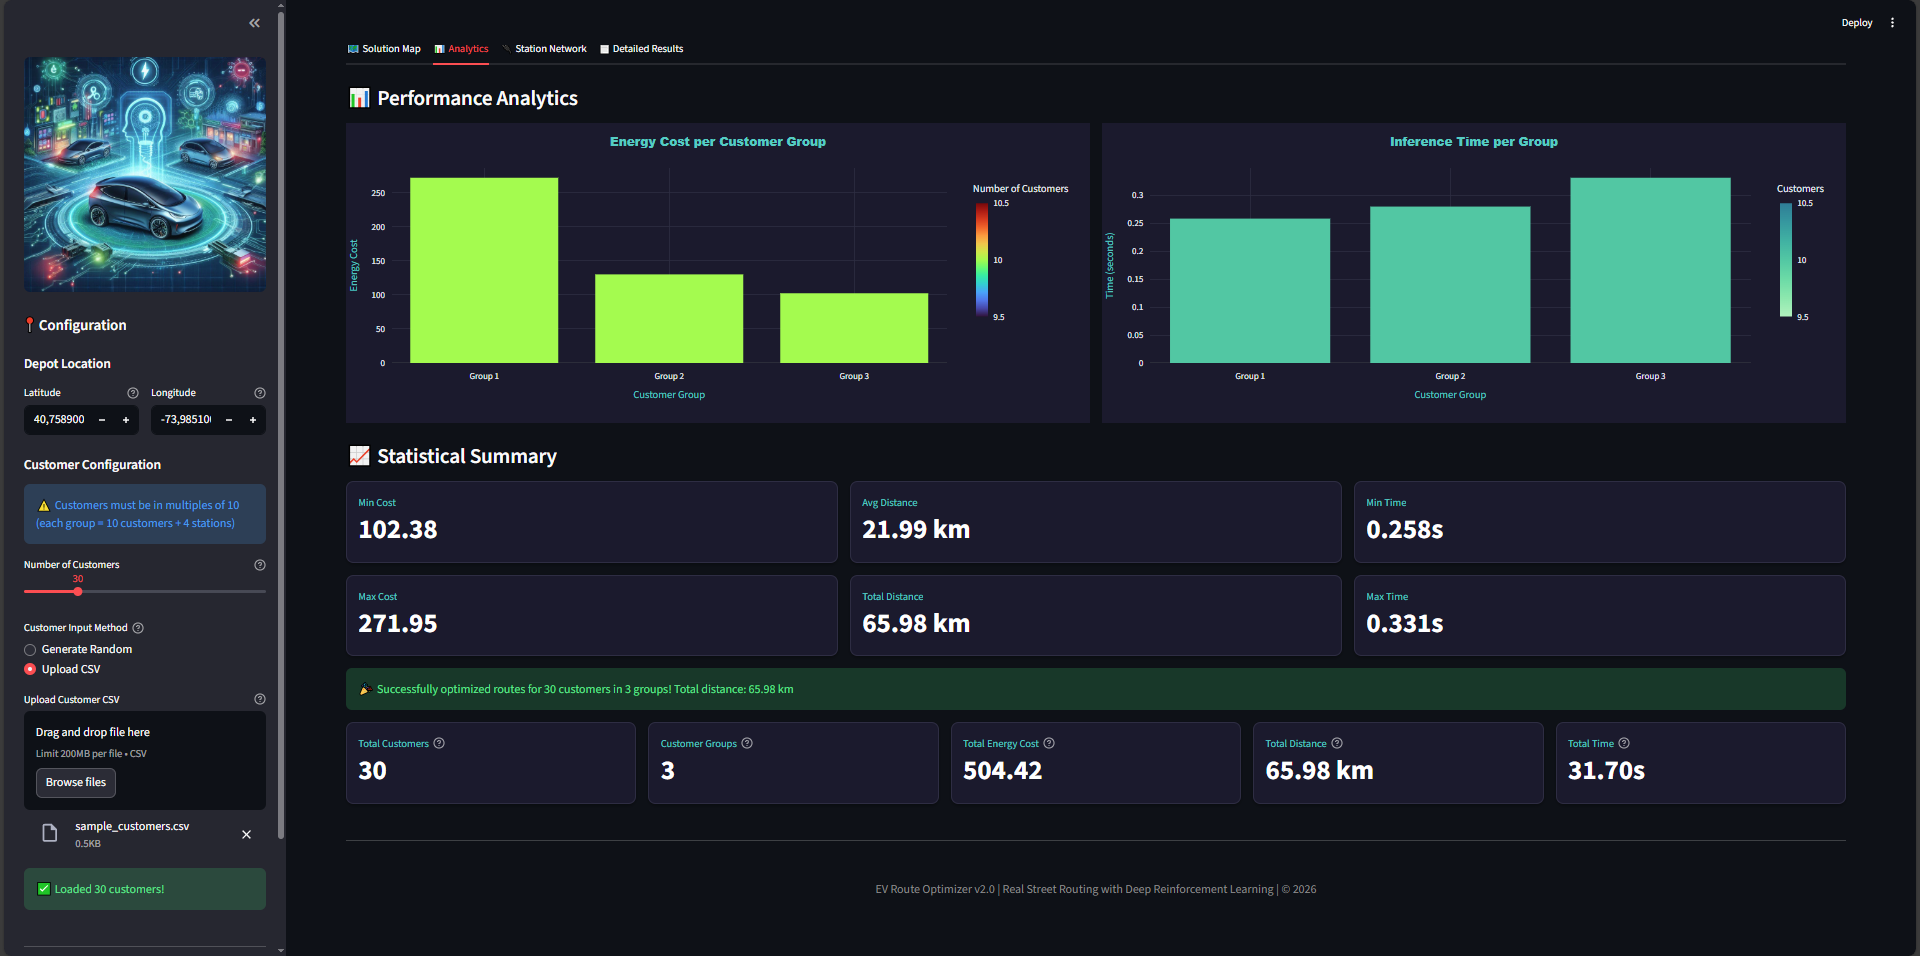
\includegraphics[width=\textwidth]{analytics.PNG}
            \end{center}
        \end{column}
        \begin{column}{0.48\textwidth}
            \begin{center}
                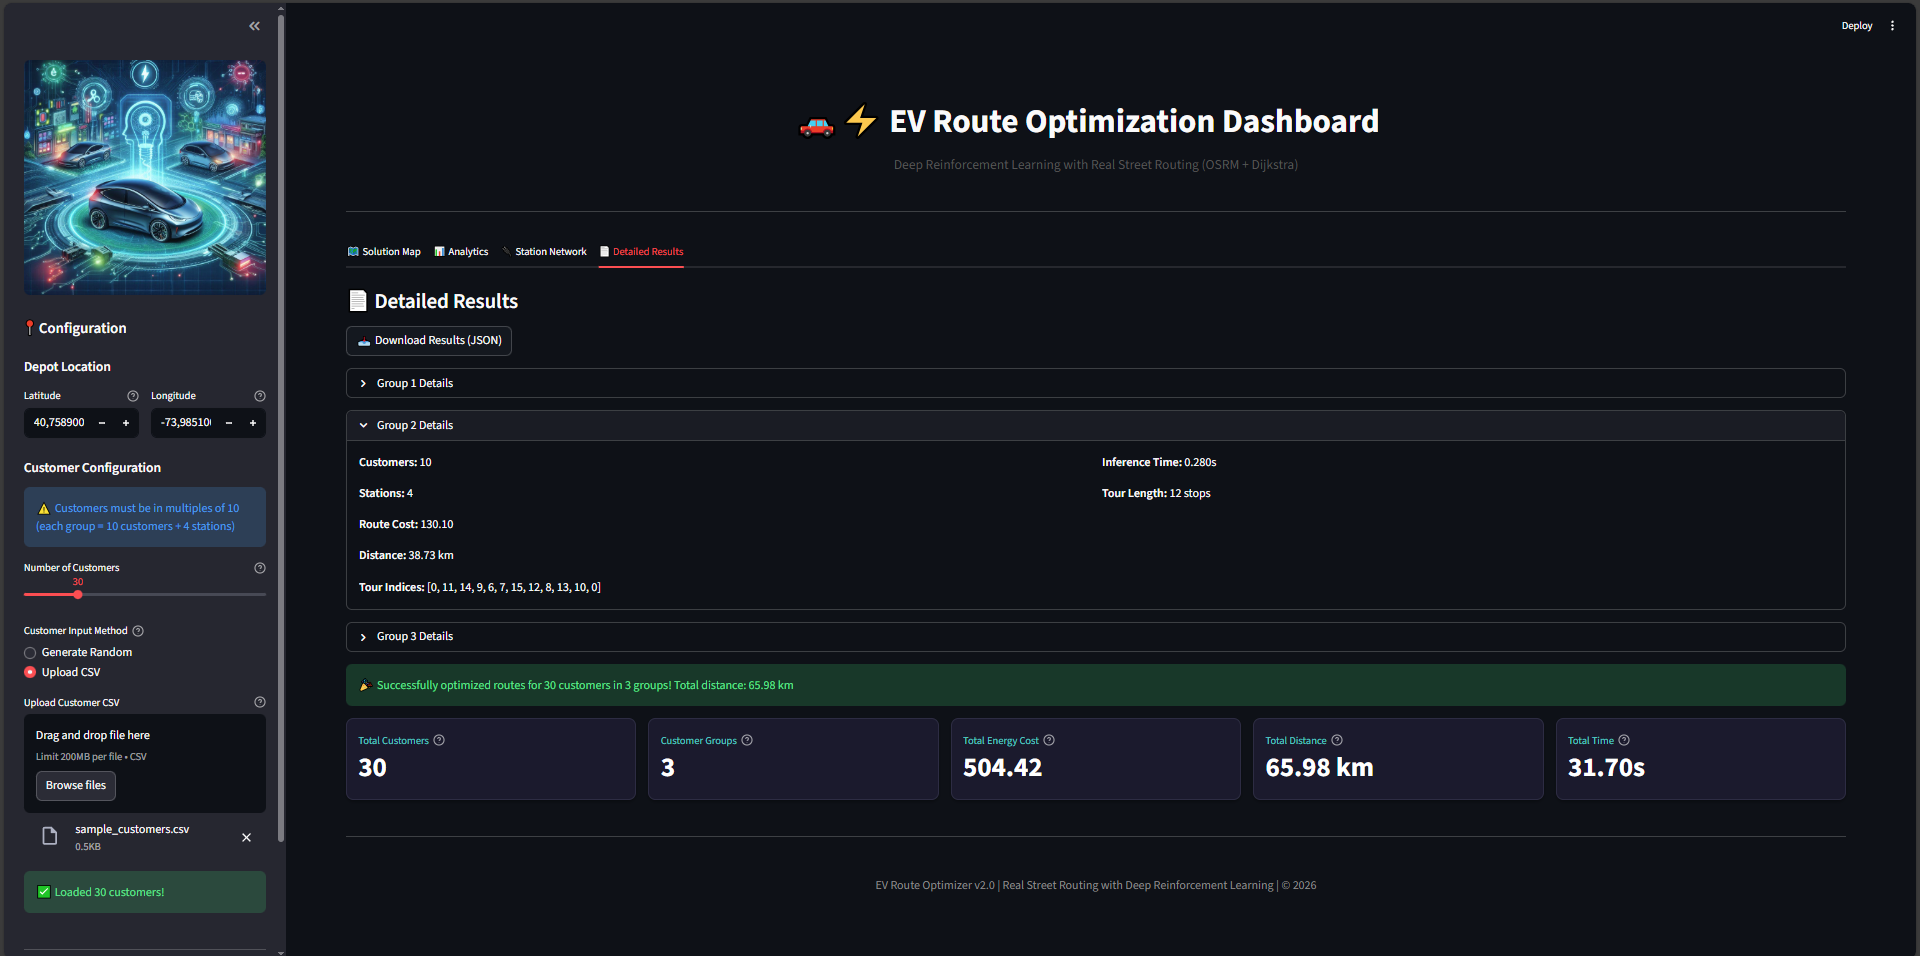
\includegraphics[width=\textwidth]{detailed.PNG}
            \end{center}
        \end{column}
    \end{columns}
    
    \vspace{0.3cm}
    \begin{block}{Analytics Features}
        \begin{itemize}
            \item Energy consumption breakdown per route segment
            \item SOC tracking throughout the journey
            \item Cost analysis and performance metrics
            \item Export results as JSON for integration
        \end{itemize}
    \end{block}
\end{frame}

%=========================================================================
\section{Results and Evaluation}
%=========================================================================

%-------------------------------------------------------------------------
\begin{frame}{Training Configuration}
    \begin{columns}[T]
        \begin{column}{0.48\textwidth}
            \begin{block}{Problem Configuration}
                \begin{tabular}{ll}
                    Customers & 10 \\
                    Charging stations & 4 \\
                    Sequence length & 16 \\
                    Initial SOC & 80\% \\
                    Max load & 50 units
                \end{tabular}
            \end{block}
            
            \begin{block}{Training Parameters}
                \begin{tabular}{ll}
                    Epochs & 20 \\
                    Batch size & 1,024 \\
                    Training samples & 1,280,000 \\
                    Learning rate & $10^{-4}$ \\
                    Baseline & Rollout
                \end{tabular}
            \end{block}
        \end{column}
        \begin{column}{0.48\textwidth}
            \begin{block}{Model Architecture}
                \begin{tabular}{ll}
                    Embedding dim & 128 \\
                    Encoder layers & 3 \\
                    Attention heads & 8 \\
                    FF hidden & 512 \\
                    Tanh clipping & 10 \\
                    Optimizer & Adam
                \end{tabular}
            \end{block}
            
            \begin{block}{Hardware}
                \begin{tabular}{ll}
                    GPU & NVIDIA RTX \\
                    Training time & $\sim$8 hours
                \end{tabular}
            \end{block}
        \end{column}
    \end{columns}
\end{frame}

%-------------------------------------------------------------------------
\begin{frame}{Training Results}
    \begin{center}
        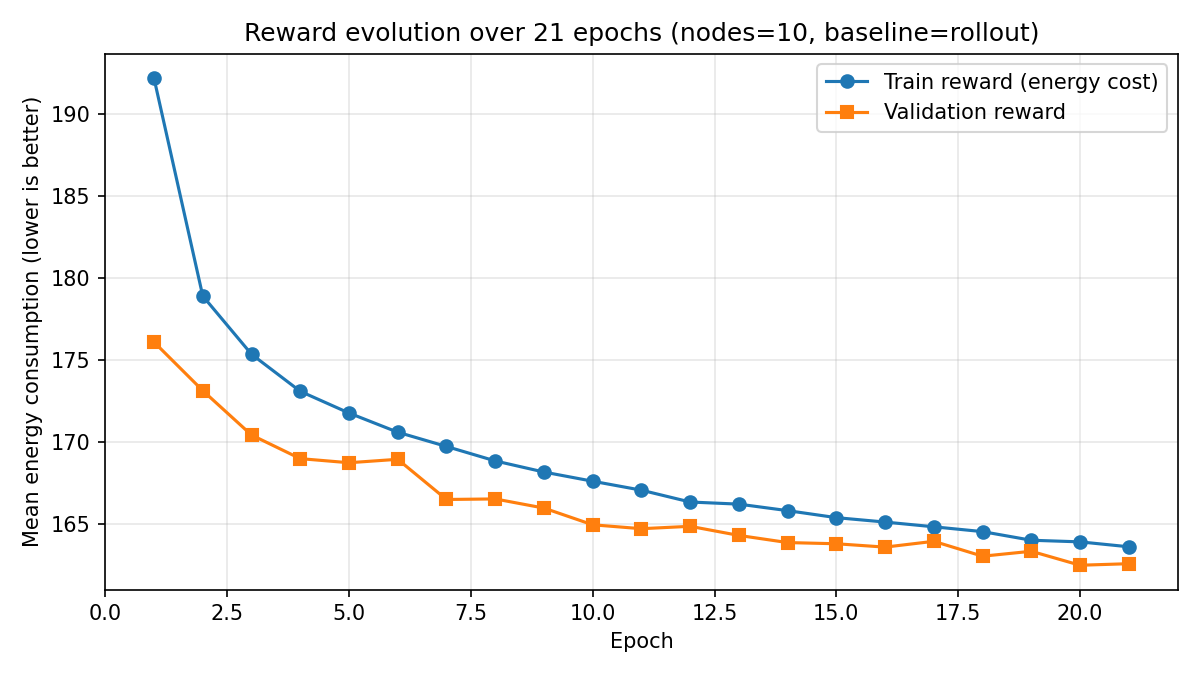
\includegraphics[width=0.7\textwidth]{training_reward.png}
    \end{center}
    
    \begin{columns}[T]
        \begin{column}{0.48\textwidth}
            \begin{block}{Training Observations}
                \begin{itemize}
                    \item Consistent improvement
                    \item Convergence around epoch 80
                    \item Low variance after convergence
                \end{itemize}
            \end{block}
        \end{column}
        \begin{column}{0.48\textwidth}
            \begin{block}{Generalization}
                \begin{itemize}
                    \item Validation follows training
                    \item No overfitting observed
                    \item Good transfer to test instances
                \end{itemize}
            \end{block}
        \end{column}
    \end{columns}
\end{frame}

%-------------------------------------------------------------------------
\begin{frame}{Performance Comparison}
    \begin{center}
        \begin{tabular}{lcc}
            \toprule
            \textbf{Method} & \textbf{Energy (kWh)} & \textbf{Inference Time} \\
            \midrule
            Google OR-Tools & 12.45 & 2.1s \\
            Hill Climbing & 13.21 & 0.8s \\
            Simulated Annealing & 12.89 & 1.5s \\
            Ant Colony Optimization & 12.67 & 3.2s \\
            \midrule
            \textbf{DRL (Ours)} & \textbf{12.18} & \textbf{0.5s} \\
            \bottomrule
        \end{tabular}
    \end{center}
    
    \vspace{0.5cm}
    \begin{columns}[T]
        \begin{column}{0.48\textwidth}
            \begin{exampleblock}{Energy Reduction}
                \begin{itemize}
                    \item \textbf{2.2\%} better than OR-Tools
                    \item \textbf{7.8\%} better than Hill Climbing
                    \item Best overall energy efficiency
                \end{itemize}
            \end{exampleblock}
        \end{column}
        \begin{column}{0.48\textwidth}
            \begin{exampleblock}{Speed Improvement}
                \begin{itemize}
                    \item \textbf{4x} faster than OR-Tools
                    \item \textbf{6x} faster than ACO
                    \item Real-time capable
                \end{itemize}
            \end{exampleblock}
        \end{column}
    \end{columns}
\end{frame}

%-------------------------------------------------------------------------
\begin{frame}{Key Findings}
    \begin{columns}[T]
        \begin{column}{0.48\textwidth}
            \begin{block}{Model Performance}
                \begin{itemize}
                    \item \cmark~Generalizes to unseen instances
                    \item \cmark~Competitive solution quality
                    \item \cmark~Significantly faster inference
                    \item \cmark~Learns charging decisions
                \end{itemize}
            \end{block}
            
            \begin{block}{Energy Model Insights}
                \begin{itemize}
                    \item Load-dependent consumption
                    \item Regenerative braking benefits
                    \item Elevation-aware routing
                \end{itemize}
            \end{block}
        \end{column}
        \begin{column}{0.48\textwidth}
            \begin{block}{Architecture Effectiveness}
                \begin{itemize}
                    \item Attention captures relationships
                    \item Context embedding is crucial
                    \item Masking ensures feasibility
                \end{itemize}
            \end{block}
            
            \begin{block}{Practical Benefits}
                \begin{itemize}
                    \item Ready for deployment
                    \item Interactive visualization
                    \item Real street routing
                    \item Scalable to larger problems
                \end{itemize}
            \end{block}
        \end{column}
    \end{columns}
\end{frame}

%=========================================================================
\section{Conclusion}
%=========================================================================

%-------------------------------------------------------------------------
\begin{frame}{Summary of Contributions}
    \begin{enumerate}
        \item \textbf{Comprehensive MILP Formulation}
        \begin{itemize}
            \item Physics-based energy consumption model
            \item Multi-trip capability with time windows
            \item Regenerative braking consideration
        \end{itemize}
        
        \vspace{0.3cm}
        \item \textbf{Baseline Implementation}
        \begin{itemize}
            \item OR-Tools, Hill Climbing, SA, ACO
            \item Standardized benchmarking framework
        \end{itemize}
        
        \vspace{0.3cm}
        \item \textbf{Deep Reinforcement Learning Solution}
        \begin{itemize}
            \item Attention-based encoder-decoder
            \item EV-specific state representation
            \item Fast and generalizable
        \end{itemize}
        
        \vspace{0.3cm}
        \item \textbf{Production-Ready System}
        \begin{itemize}
            \item Interactive Streamlit dashboard
            \item OSRM integration for real streets
            \item Export and analytics features
        \end{itemize}
    \end{enumerate}
\end{frame}

%-------------------------------------------------------------------------
\begin{frame}{Limitations and Future Work}
    \begin{columns}[T]
        \begin{column}{0.48\textwidth}
            \begin{alertblock}{Current Limitations}
                \begin{itemize}
                    \item Trained on 10 customers
                    \item Single depot scenario
                    \item Homogeneous fleet
                    \item Static demand
                    \item No traffic dynamics
                \end{itemize}
            \end{alertblock}
        \end{column}
        \begin{column}{0.48\textwidth}
            \begin{exampleblock}{Future Directions}
                \begin{itemize}
                    \item Scale to 50+ customers
                    \item Multi-depot extension
                    \item Heterogeneous EV types
                    \item Dynamic reoptimization
                    \item Real-time traffic integration
                    \item Joint routing + charging scheduling
                \end{itemize}
            \end{exampleblock}
        \end{column}
    \end{columns}
    
    \vspace{0.5cm}
    \begin{block}{Research Extensions}
        \begin{itemize}
            \item Transfer learning for larger instances
            \item Multi-agent coordination for fleet management
            \item Integration with smart grid for optimal charging times
        \end{itemize}
    \end{block}
\end{frame}

%-------------------------------------------------------------------------
\begin{frame}{Conclusion}
    \begin{center}
        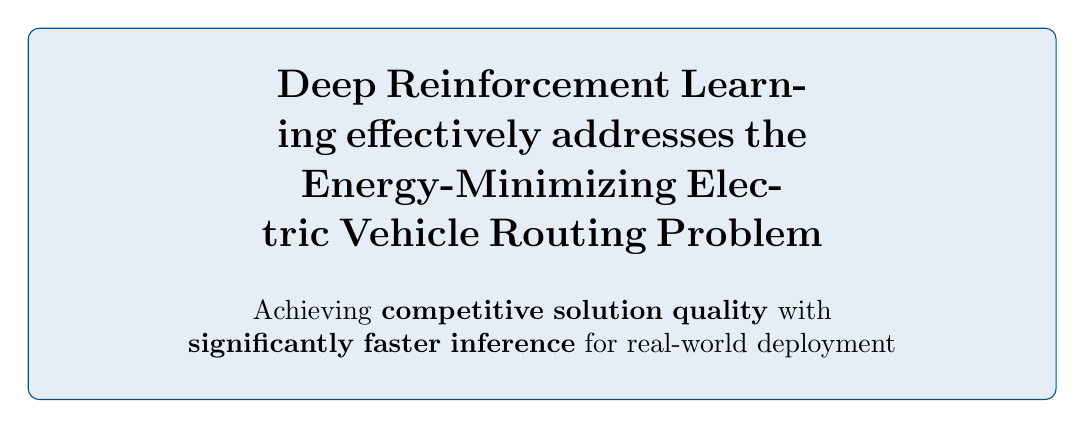
\begin{tikzpicture}
            \node[rectangle, rounded corners, draw=primaryblue, fill=primaryblue!10, 
                  text width=12cm, align=center, inner sep=15pt] {
                \Large\textbf{Deep Reinforcement Learning effectively addresses the\\
                Energy-Minimizing Electric Vehicle Routing Problem}\\[0.5cm]
                \normalsize
                Achieving \textbf{competitive solution quality} with\\
                \textbf{significantly faster inference} for real-world deployment
            };
        \end{tikzpicture}
    \end{center}
    
    \vspace{0.5cm}
    \begin{columns}[T]
        \begin{column}{0.32\textwidth}
            \centering
            \faIcon{brain}\\
            \textbf{Learning-Based}\\
            Generalizes to new instances
        \end{column}
        \begin{column}{0.32\textwidth}
            \centering
            \faIcon{bolt}\\
            \textbf{Energy-Efficient}\\
            Physics-aware optimization
        \end{column}
        \begin{column}{0.32\textwidth}
            \centering
            \faIcon{rocket}\\
            \textbf{Production-Ready}\\
            Interactive dashboard
        \end{column}
    \end{columns}
\end{frame}

%-------------------------------------------------------------------------
\begin{frame}[plain]
    \begin{center}
        \vspace{2cm}
        {\Huge\textbf{Thank You!}}
        
        \vspace{1cm}
        {\Large Questions \& Discussion}
        
        \vspace{1.5cm}
        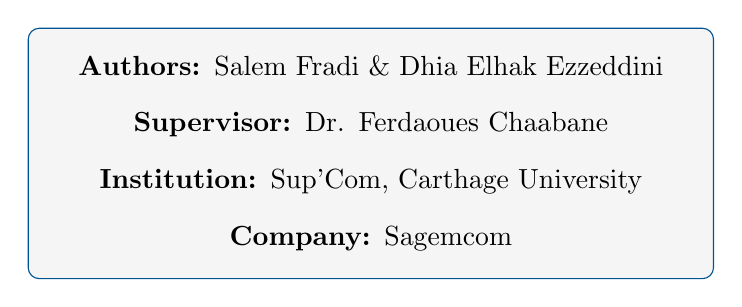
\begin{tikzpicture}
            \node[rectangle, rounded corners, draw=primaryblue, fill=lightgray, 
                  text width=8cm, align=center, inner sep=10pt] {
                \textbf{Authors:} Salem Fradi \& Dhia Elhak Ezzeddini\\[0.3cm]
                \textbf{Supervisor:} Dr. Ferdaoues Chaabane\\[0.3cm]
                \textbf{Institution:} Sup'Com, Carthage University\\[0.3cm]
                \textbf{Company:} Sagemcom
            };
        \end{tikzpicture}
        
        \vspace{1cm}
        {\large Academic Year 2025--2026}
    \end{center}
\end{frame}

%-------------------------------------------------------------------------
% BACKUP SLIDES
%-------------------------------------------------------------------------
\appendix
\begin{frame}{Backup: Node Indexing Convention}
    \begin{block}{Sequence Layout (10 customers, 4 stations)}
        \begin{tabular}{cl}
            \toprule
            \textbf{Index} & \textbf{Node Type} \\
            \midrule
            0 & Depot \\
            1 & Depot charging (near depot) \\
            2--5 & Charging stations (4 stations) \\
            6--15 & Customers (10 customers) \\
            \bottomrule
        \end{tabular}
    \end{block}
    
    \vspace{0.5cm}
    \textbf{Total sequence length:} $2 + 4 + 10 = 16$ nodes
    
    \vspace{0.3cm}
    \textbf{Dynamic state tensor:} 4 channels
    \begin{itemize}
        \item Load: remaining capacity
        \item Demand: per-node remaining demand
        \item SOC: battery state of charge
        \item Time: remaining route time budget
    \end{itemize}
\end{frame}

%-------------------------------------------------------------------------
\begin{frame}{Backup: Masking Logic Details}
    \textbf{Feasibility conditions applied sequentially:}
    
    \begin{enumerate}
        \item Base feasibility: demand $> 0$ AND demand $<$ current load
        \item Previously selected node is masked
        \item Charging access restrictions based on current location
        \item Force depot return if no load OR no remaining demand
        \item Block nodes unreachable due to SOC or time
        \item Block if two-leg path to depot infeasible
        \item Ensure depot always selectable when all customers masked
    \end{enumerate}
    
    \vspace{0.3cm}
    \begin{exampleblock}{Purpose}
        Ensures energy, time, load, and demand constraints while\\
        permitting charging detours and driving termination
    \end{exampleblock}
\end{frame}

%-------------------------------------------------------------------------
\begin{frame}{Backup: References}
    \begin{thebibliography}{9}
        \bibitem{kool}
        W. Kool, H. van Hoof, M. Welling,
        \textit{``Attention, Learn to Solve Routing Problems!''},
        ICLR, 2019.
        
        \bibitem{osrm}
        Project OSRM - Open Source Routing Machine.
        \url{http://project-osrm.org/}
        
        \bibitem{ortools}
        Google OR-Tools.
        \url{https://developers.google.com/optimization}
        
        \bibitem{cvrplib}
        CVRPLIB: Capacitated Vehicle Routing Problem Library.
        \url{http://vrp.atd-lab.inf.puc-rio.br/}
        
        \bibitem{vaswani}
        A. Vaswani et al.,
        \textit{``Attention Is All You Need''},
        NeurIPS, 2017.
    \end{thebibliography}
\end{frame}

\end{document}
